\documentclass[10pt,UTF8]{book} %% ctexart

\title{\textbf{计算机网络}}
\author{钱锋\thanks{Email: strik0r.qf@gmail.com}${}^,$\thanks{
    西北工业大学软件学院, School of Software, Northwestern Polytechnical University, 西安 710072
}}

\usepackage{ctex}
\usepackage{graphicx}
\usepackage[toc]{multitoc}
\usepackage{amsthm, amssymb, amsmath, mathrsfs, mhchem}
\usepackage{tikz,circuitikz}
\usetikzlibrary{decorations.markings, angles, quotes, arrows.meta, er}
\usepackage{pgfplots}
\usepackage{subcaption}
\usepackage{tikz-3dplot}
\usepackage{extpfeil}
\usepackage{diagbox}
\usepackage{float}
\usepackage{hyperref}
\hypersetup{hidelinks,
    colorlinks = true,
    allcolors = black,
    pdfstartview = Fit,
    breaklinks = true}
\usepackage{caption}
\usepackage{enumitem}
\usepackage{siunitx}
% 定义带圆圈的数字命令
\newcommand{\circled}[1]{\textcircled{\small #1}}

\usepackage{fancyhdr} % 用于自定义页眉页脚


% 设置页眉页脚样式
\fancypagestyle{plain}{%
    \fancyhf{} % 清空页眉页脚
    \fancyhead[RO,LE]{·\thepage·} % 页眉显示页码, RO表示奇数页右侧, LE表示偶数页左侧
    \fancyhead[LO]{\nouppercase{\rightmark}} % 页眉显示小节标题, LO表示奇数页左侧
    \fancyhead[RE]{\nouppercase{\leftmark}} % 页眉显示章节标题, RE表示偶数页右侧
    \renewcommand{\headrulewidth}{0.4pt} % 设置页眉横线的宽度
    \renewcommand{\footrulewidth}{0pt} % 取消页脚横线
}

\renewcommand{\headrule}{\hrule width\textwidth height\headrulewidth\vskip-\headrulewidth}

% % 取消奇偶页的页眉偏移
% \fancyhfoffset[RO,LE]{0pt}

% % 取消奇偶页的页眉偏移
% \fancyhfoffset[RO,LE]{0pt}

% 定义取消页眉的命令
\newcommand{\cancelheader}{%
    \fancyhead{} % 清空页眉
    \renewcommand{\headrulewidth}{0pt} % 取消页眉横线
    \renewcommand{\footrulewidth}{0pt} % 设置页脚横线的宽度
}

\renewcommand{\chaptermark}[1]{\markboth{第 \thechapter 章 \hspace{1em} #1}{}}
\renewcommand{\sectionmark}[1]{\markright{\thesection \, #1}}
\usepackage{titlesec} % 定义标题样式

% 设置 chapter 标题样式
\titleformat{\chapter}[hang]{\centering\heiti\Large\bfseries}{第\,\thechapter\,章}{1em}{}

% 定义 section 标题格式
\titleformat{\section}[hang]{\heiti\centering\large\bfseries}{\thesection}{1em}{}

% 定义 subsection 标题格式
\titleformat{\subsection}[hang]{\heiti\bfseries}{\textbf{\thesubsection}}{1em}{}

% 定义 subsubsection 标题格式
\setcounter{secnumdepth}{3}
\renewcommand\thesubsubsection{\arabic{subsubsection}.}
\titleformat{\subsubsection}[hang]{\kaishu}{\quad\quad\thesubsubsection\,\,}{0em}{}

% % 重新定义 textbf
% \let\oldtextbf\textbf
% \renewcommand{\textbf}[1]{{\heiti\oldtextbf{#1}}}

% % 在导言区重新定义 \normalsize 命令
% \makeatletter
% \renewcommand\normalsize{%
%    \@setfontsize\normalsize{10.5pt}{12pt}%
%    \abovedisplayskip 8\p@ \@plus2\p@ \@minus5\p@
%    \abovedisplayshortskip \z@ \@plus3\p@
%    \belowdisplayshortskip 6\p@ \@plus3\p@ \@minus3\p@
%    \belowdisplayskip \abovedisplayskip
%    \let\@listi\@listI}
% \makeatother



% 设置页边距和对齐
% \usepackage[
%     paperwidth=185mm,
%     paperheight=260mm,
%     top=35mm,
%     bottom=25mm,
%     left=18mm,
%     right=18mm,
%     footskip=15mm % 通过这里的值来调整页脚与正文内容的垂直距离
% ]{geometry}

\usepackage[
    paperwidth=210mm,
    paperheight=297mm,
    top=40mm,
    bottom=31.8mm,
    left=25.4mm,
    right=25.4mm,
    footskip=15mm % 通过这里的值来调整页脚与正文内容的垂直距离
]{geometry}

% \usepackage[
%     paperwidth=195mm,
%     paperheight=270mm,
%     top=40mm,
%     bottom=25mm,
%     left=23.5mm,
%     right=23.5mm,
%     footskip=15mm % 通过这里的值来调整页脚与正文内容的垂直距离
% ]{geometry}
\usepackage{mdframed}
\mdfsetup{
  linewidth=0.4pt,
  frametitlebackgroundcolor=white, % 或者 transparent
  frametitlefont=\heiti\bfseries,
  frametitleaboveskip=10pt,
  frametitlebelowskip=5pt,
  frametitlealignment=\raggedright % 新增此行
}
\usepackage{fontspec}
% 设置 Menlo 字体
\setmonofont{Menlo}
\usepackage{fancyvrb}
\usepackage{xcolor}
\usepackage{listings}

% \definecolor{string}{HTML}{067D17}
% \definecolor{comment}{HTML}{8C8C8C}
% \definecolor{keyword}{HTML}{0033B3}
% \definecolor{class_field}{HTML}{871094}

\lstset{breaklines}
%这条命令可以让LaTeX自动将长的代码行换行排版
\lstset{extendedchars=false}
%这一条命令可以解决代码跨页时,章节标题,页眉等汉字不显示的问题
\lstset{escapeinside={(*}{*)}}

\lstset{
    basicstyle=\small\ttfamily\heiti,
    numbers=left,
    numberstyle=\scriptsize\fontspec{Menlo}, % 使用 Menlo 字体
    stepnumber=1,
    numbersep=8pt,
    frame=leftline,
    xleftmargin=2em, % 调整代码块的左边界
    framexleftmargin=0pt, % 调整边框的位置
    breaklines=true,
    % postbreak=\mbox{\textcolor{red}{$\hookrightarrow$}\space},
    % keywordstyle=\bfseries\color{keyword},          % keyword style
    % commentstyle=\heiti\color{comment},       % comment style
    % stringstyle=\color[HTML]{067D17},
    showstringspaces=false,
    % string literal style
    % escapeinside={\%*}{*)},            % if you want to add LaTeX within your code
    % morekeywords={}               % if you want to add more keywords to the set
}

\usepackage{smartdiagram}
\usepackage{subcaption}
\usepackage{tasks}
\everymath{\displaystyle}

\begin{document}

\newtheoremstyle{mytheoremstyle}
    {1.5ex}                                         % Space above
    {1.5ex}                                         % Space below
    {}                                              % Font for body
    {}                                              % Indent amount
    {\bfseries}                                     % Font for head
    {}                                              % Punctuation after head
    {0.5em plus 0.2em minus 0.1em}                  % Space after head
    {\thmname{#1}\thmnumber{ #2}.\thmnote{ (#3).}}

\theoremstyle{mytheoremstyle}
\newtheorem{definition}{定义}[section]
\newtheorem{example}{例}[section]
\newtheorem{exercise}{习题}[section]
\newtheorem{code}{程序清单}[section]
\newtheorem*{result}{运行结果}

\newtheoremstyle{my2theoremstyle}
    {1.5ex}                                         % Space above
    {1.5ex}                                         % Space below
    {\kaishu}                                              % Font for body
    {}                                              % Indent amount
    {\bfseries}                                     % Font for head
    {}                                              % Punctuation after head
    {0.5em plus 0.2em minus 0.1em}                  % Space after head
    {\thmname{#1}\thmnumber{ #2}.\thmnote{ (#3).}}

\theoremstyle{my2theoremstyle}
\newtheorem{thm}{定理}[section]
\newtheorem{law}{定律}[section]
\newtheorem{educt}{推论}
\newtheorem{prop}{命题}
\newtheorem{lemma}{引理}
\newtheorem{axiom}{公理}
\newtheorem{property}{性质}

\newtheoremstyle{my4theoremstyle}
    {1.5ex}                                         % Space above
    {1.5ex}                                         % Space below
    {}                                              % Font for body
    {}                                              % Indent amount
    {\bfseries}                                     % Font for head
    {}                                              % Punctuation after head
    {0.5em plus 0.2em minus 0.1em}                  % Space after head
    {\thmname{#1}.}

\theoremstyle{my4theoremstyle} \newtheorem*{sol}{解}

\newtheoremstyle{my3theoremstyle}
    {1.5ex}                                         % Space above
    {1.5ex}                                         % Space below
    {}                                              % Font for body
    {}                                              % Indent amount
    {\kaishu}                                       % Font for head
    {}                                              % Punctuation after head
    {0.5em plus 0.2em minus 0.1em}                  % Space after head
    {\thmname{#1}\thmnumber{ #2}.\thmnote{ (#3).}}

\theoremstyle{my3theoremstyle} \newtheorem*{remark}{注}
\newtheorem*{cmt}{评注}
\pagestyle{empty}
\begin{titlepage}
    \thispagestyle{empty}
    \centering
        \vspace*{2cm}
        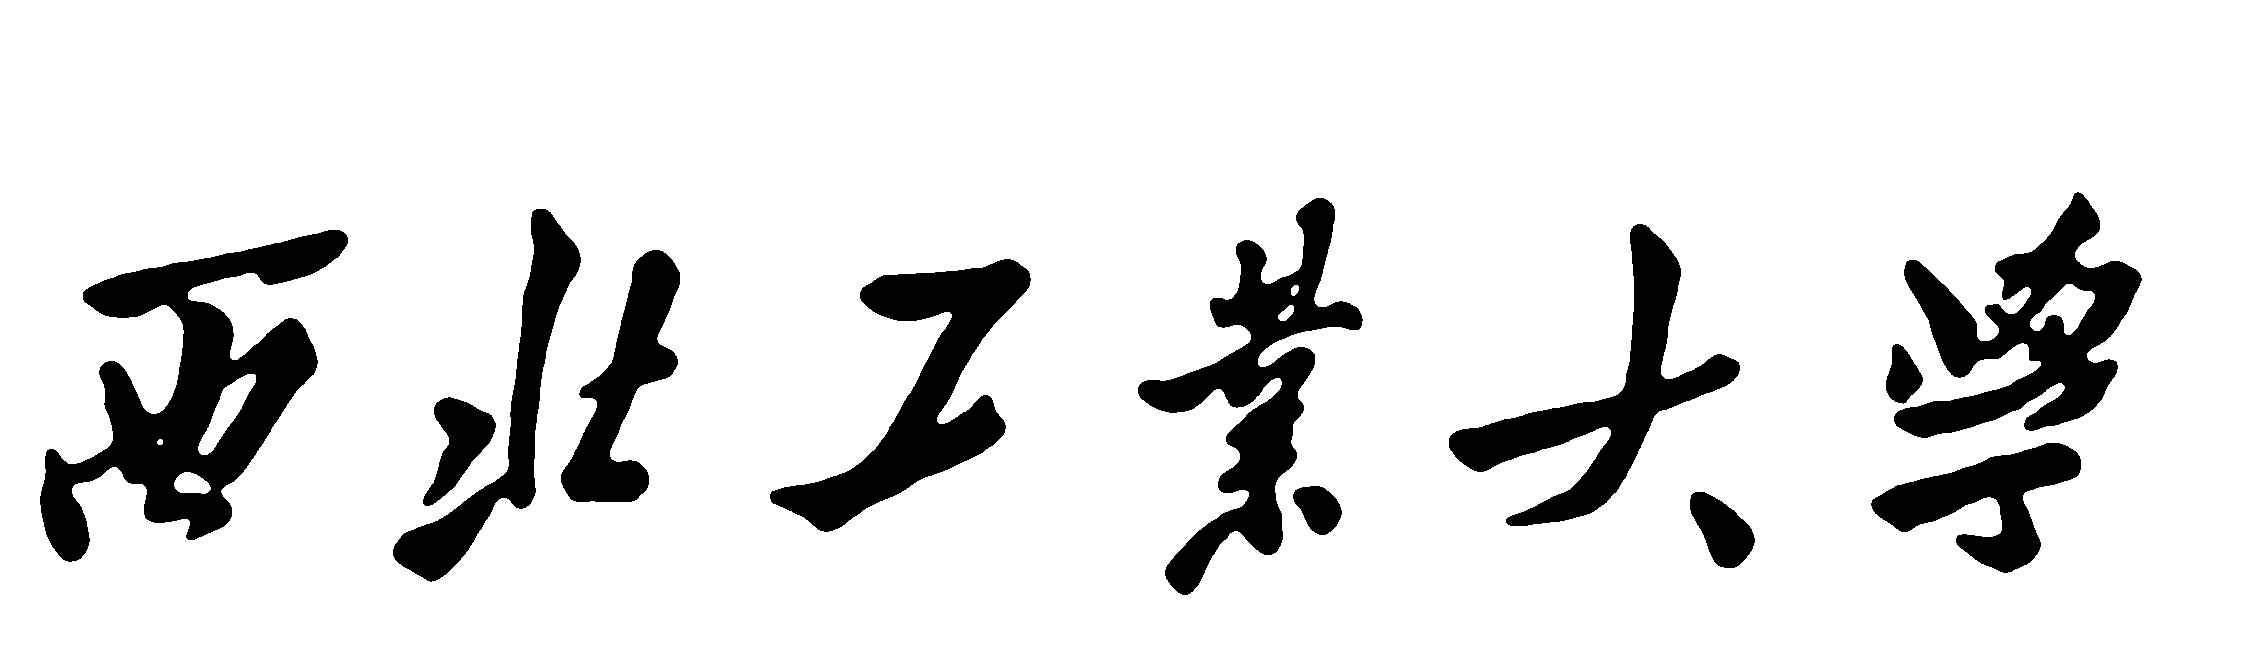
\includegraphics[width=0.5\textwidth]{pic/npu_2.png}\par
        \vspace{1em}
        
\includegraphics[width=0.5\textwidth]{pic/npu_1.png}\par
    \vspace{1cm}
        \begin{center}
            \Huge \heiti \textbf{计算机网络}

            Computer Networking
        \end{center}
        \vspace{15em}
        \begin{center}
        \songti
        \kaishu 软件学院 \, \heiti\textbf{钱锋} \quad \songti 编
        \vspace{0.5em}

    \today
    \end{center}
\end{titlepage}
\cleardoublepage
\maketitle
\cleardoublepage

\frontmatter
\newpage
\pagestyle{plain}
\makeatother

% 设置目录页的页码格式
\addtocontents{toc}{\protect\thispagestyle{empty}}
\pagestyle{plain}
{\tableofcontents}
\newpage
\thispagestyle{empty}
\cleardoublepage % 确保正文从奇数页开始


% 设置章节标题页的页眉和页脚为空白页样式
\makeatletter
\let\ps@plain\ps@empty
\makeatother

\mainmatter

\chapter{计算机网络和因特网}

\section{计算机网络概述}

\subsection{计算机网络的概念和功能}

\begin{figure}[H]
    \centering


\tikzset{every picture/.style={line width=0.75pt}} %set default line width to 0.75pt        

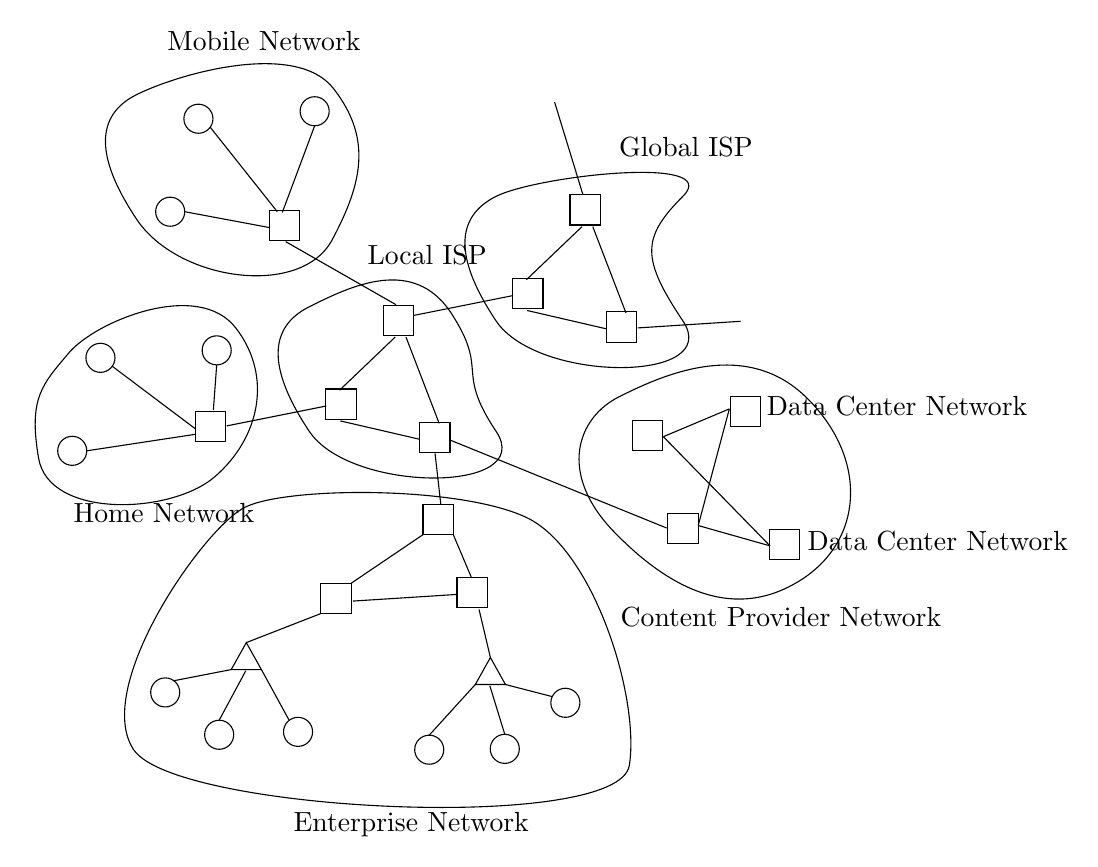
\begin{tikzpicture}[x=0.75pt,y=0.75pt,yscale=-1,xscale=1]
%uncomment if require: \path (0,424); %set diagram left start at 0, and has height of 424

%Shape: Circle [id:dp2941528290770926] 
\draw   (90.8,51.4) .. controls (90.8,47.53) and (93.93,44.4) .. (97.8,44.4) .. controls (101.67,44.4) and (104.8,47.53) .. (104.8,51.4) .. controls (104.8,55.27) and (101.67,58.4) .. (97.8,58.4) .. controls (93.93,58.4) and (90.8,55.27) .. (90.8,51.4) -- cycle ;
%Shape: Circle [id:dp0009345117077476095] 
\draw   (77.2,96.2) .. controls (77.2,92.33) and (80.33,89.2) .. (84.2,89.2) .. controls (88.07,89.2) and (91.2,92.33) .. (91.2,96.2) .. controls (91.2,100.07) and (88.07,103.2) .. (84.2,103.2) .. controls (80.33,103.2) and (77.2,100.07) .. (77.2,96.2) -- cycle ;
%Shape: Circle [id:dp530616605018679] 
\draw   (146.8,47.8) .. controls (146.8,43.93) and (149.93,40.8) .. (153.8,40.8) .. controls (157.67,40.8) and (160.8,43.93) .. (160.8,47.8) .. controls (160.8,51.67) and (157.67,54.8) .. (153.8,54.8) .. controls (149.93,54.8) and (146.8,51.67) .. (146.8,47.8) -- cycle ;
%Shape: Square [id:dp4877040359362528] 
\draw   (132,95.6) -- (146.6,95.6) -- (146.6,110.2) -- (132,110.2) -- cycle ;
%Straight Lines [id:da030713204061328603] 
\draw    (91.2,96.2) -- (131.8,103.8) ;
%Straight Lines [id:da11845760953458018] 
\draw    (103.4,55.4) -- (135.8,96.2) ;
%Straight Lines [id:da28899851098805696] 
\draw    (153.8,54.8) -- (138.2,96.6) ;
%Shape: Square [id:dp5502568063339528] 
\draw   (186.8,141.2) -- (201.4,141.2) -- (201.4,155.8) -- (186.8,155.8) -- cycle ;
%Shape: Square [id:dp440732274708848] 
\draw   (159.2,181.6) -- (173.8,181.6) -- (173.8,196.2) -- (159.2,196.2) -- cycle ;
%Shape: Square [id:dp8144918506695862] 
\draw   (204.4,197.6) -- (219,197.6) -- (219,212.2) -- (204.4,212.2) -- cycle ;
%Shape: Polygon Curved [id:ds8887635795146563] 
\draw   (68,39.8) .. controls (88,29.8) and (144.8,13.4) .. (163,37) .. controls (181.2,60.6) and (177.2,81.8) .. (162.2,109.8) .. controls (147.2,137.8) and (88,129.8) .. (68,99.8) .. controls (48,69.8) and (48,49.8) .. (68,39.8) -- cycle ;
%Shape: Polygon Curved [id:ds8983519342294061] 
\draw   (151.2,142) .. controls (171.2,132) and (201.6,117.2) .. (219.8,145.4) .. controls (238,173.6) and (221.2,172) .. (241.2,202) .. controls (261.2,232) and (171.2,232) .. (151.2,202) .. controls (131.2,172) and (131.2,152) .. (151.2,142) -- cycle ;
%Straight Lines [id:da923538035744028] 
\draw    (192.6,156.6) -- (165.8,182.2) ;
%Straight Lines [id:da3573057000836749] 
\draw    (197.8,156.6) -- (213.8,198.2) ;
%Straight Lines [id:da3909626127490258] 
\draw    (166.2,197) -- (204.2,205.8) ;
%Shape: Circle [id:dp9962102527174099] 
\draw   (43.6,166.6) .. controls (43.6,162.73) and (46.73,159.6) .. (50.6,159.6) .. controls (54.47,159.6) and (57.6,162.73) .. (57.6,166.6) .. controls (57.6,170.47) and (54.47,173.6) .. (50.6,173.6) .. controls (46.73,173.6) and (43.6,170.47) .. (43.6,166.6) -- cycle ;
%Shape: Circle [id:dp14683096883897018] 
\draw   (30,211.4) .. controls (30,207.53) and (33.13,204.4) .. (37,204.4) .. controls (40.87,204.4) and (44,207.53) .. (44,211.4) .. controls (44,215.27) and (40.87,218.4) .. (37,218.4) .. controls (33.13,218.4) and (30,215.27) .. (30,211.4) -- cycle ;
%Shape: Circle [id:dp7305194827842264] 
\draw   (99.6,163) .. controls (99.6,159.13) and (102.73,156) .. (106.6,156) .. controls (110.47,156) and (113.6,159.13) .. (113.6,163) .. controls (113.6,166.87) and (110.47,170) .. (106.6,170) .. controls (102.73,170) and (99.6,166.87) .. (99.6,163) -- cycle ;
%Shape: Square [id:dp14290049737961275] 
\draw   (96.4,192.4) -- (111,192.4) -- (111,207) -- (96.4,207) -- cycle ;
%Straight Lines [id:da7116349195714726] 
\draw    (44,211.4) -- (96.6,203.4) ;
%Straight Lines [id:da3217533313879044] 
\draw    (56.2,170.6) -- (96.6,201) ;
%Straight Lines [id:da4033262026488128] 
\draw    (106.6,170) -- (105,191.8) ;
%Shape: Polygon Curved [id:ds050162825089125285] 
\draw   (35.4,164.2) .. controls (48.2,149) and (97.6,128.6) .. (115.8,152.2) .. controls (134,175.8) and (127,205.4) .. (105.8,223.8) .. controls (84.6,242.2) and (25.8,244.2) .. (20.8,215) .. controls (15.8,185.8) and (22.6,179.4) .. (35.4,164.2) -- cycle ;
%Straight Lines [id:da752186888557205] 
\draw    (139.8,110.6) -- (193,141) ;
%Straight Lines [id:da4788480105895748] 
\draw    (111.4,199.4) -- (159.4,189.8) ;
%Shape: Square [id:dp46873093708859936] 
\draw   (206,237.2) -- (220.6,237.2) -- (220.6,251.8) -- (206,251.8) -- cycle ;
%Shape: Square [id:dp3825236294915455] 
\draw   (156.8,275.2) -- (171.4,275.2) -- (171.4,289.8) -- (156.8,289.8) -- cycle ;
%Shape: Square [id:dp4556416728273698] 
\draw   (222.4,272.4) -- (237,272.4) -- (237,287) -- (222.4,287) -- cycle ;
%Straight Lines [id:da6213703493867873] 
\draw    (171.4,275.2) -- (206,251.8) ;
%Straight Lines [id:da11017130641127126] 
\draw    (229.4,272.6) -- (220.6,251.8) ;
%Straight Lines [id:da18944670974892275] 
\draw    (222.2,280.6) -- (172.2,283.8) ;
%Straight Lines [id:da694521923861742] 
\draw    (211.8,212.6) -- (214.6,237.4) ;
%Flowchart: Extract [id:dp8208973782779554] 
\draw   (120.87,303.8) -- (128.14,316.8) -- (113.6,316.8) -- cycle ;
%Shape: Circle [id:dp06456973906298236] 
\draw   (74.8,327.8) .. controls (74.8,323.93) and (77.93,320.8) .. (81.8,320.8) .. controls (85.67,320.8) and (88.8,323.93) .. (88.8,327.8) .. controls (88.8,331.67) and (85.67,334.8) .. (81.8,334.8) .. controls (77.93,334.8) and (74.8,331.67) .. (74.8,327.8) -- cycle ;
%Shape: Circle [id:dp7639043168629887] 
\draw   (100.8,348.2) .. controls (100.8,344.33) and (103.93,341.2) .. (107.8,341.2) .. controls (111.67,341.2) and (114.8,344.33) .. (114.8,348.2) .. controls (114.8,352.07) and (111.67,355.2) .. (107.8,355.2) .. controls (103.93,355.2) and (100.8,352.07) .. (100.8,348.2) -- cycle ;
%Shape: Circle [id:dp4930723485080304] 
\draw   (138.8,346.8) .. controls (138.8,342.93) and (141.93,339.8) .. (145.8,339.8) .. controls (149.67,339.8) and (152.8,342.93) .. (152.8,346.8) .. controls (152.8,350.67) and (149.67,353.8) .. (145.8,353.8) .. controls (141.93,353.8) and (138.8,350.67) .. (138.8,346.8) -- cycle ;
%Straight Lines [id:da8701929222363148] 
\draw    (85.8,322.2) -- (113.6,316.8) ;
%Straight Lines [id:da6814331836855911] 
\draw    (107.8,341.2) -- (120.6,317.4) ;
%Straight Lines [id:da4761568971132447] 
\draw    (141.4,341) -- (128.14,316.8) ;
%Straight Lines [id:da9305431940351716] 
\draw    (156.8,289.8) -- (120.87,303.8) ;
%Flowchart: Extract [id:dp5351518676121784] 
\draw   (238.47,311) -- (245.74,324) -- (231.2,324) -- cycle ;
%Shape: Circle [id:dp06774089452927134] 
\draw   (202,355.4) .. controls (202,351.53) and (205.13,348.4) .. (209,348.4) .. controls (212.87,348.4) and (216,351.53) .. (216,355.4) .. controls (216,359.27) and (212.87,362.4) .. (209,362.4) .. controls (205.13,362.4) and (202,359.27) .. (202,355.4) -- cycle ;
%Shape: Circle [id:dp900792311147118] 
\draw   (238.4,355) .. controls (238.4,351.13) and (241.53,348) .. (245.4,348) .. controls (249.27,348) and (252.4,351.13) .. (252.4,355) .. controls (252.4,358.87) and (249.27,362) .. (245.4,362) .. controls (241.53,362) and (238.4,358.87) .. (238.4,355) -- cycle ;
%Shape: Circle [id:dp2615853129368638] 
\draw   (267.6,332.8) .. controls (267.6,328.93) and (270.73,325.8) .. (274.6,325.8) .. controls (278.47,325.8) and (281.6,328.93) .. (281.6,332.8) .. controls (281.6,336.67) and (278.47,339.8) .. (274.6,339.8) .. controls (270.73,339.8) and (267.6,336.67) .. (267.6,332.8) -- cycle ;
%Straight Lines [id:da7620794484414342] 
\draw    (209,348.4) -- (231.2,324) ;
%Straight Lines [id:da8409904169810318] 
\draw    (245.4,348) -- (238.2,324.6) ;
%Straight Lines [id:da37309061108562835] 
\draw    (268.2,329.8) -- (245.74,324) ;
%Straight Lines [id:da6121885569283133] 
\draw    (233,287.8) -- (238.47,311) ;
%Shape: Polygon Curved [id:ds41470221702226273] 
\draw   (120.2,238.6) .. controls (140.2,228.6) and (223,228.2) .. (255.6,243.4) .. controls (288.2,258.6) and (310.6,330.2) .. (305.4,363) .. controls (300.2,395.8) and (86.6,385.4) .. (66.6,355.4) .. controls (46.6,325.4) and (100.2,248.6) .. (120.2,238.6) -- cycle ;
%Shape: Square [id:dp9062524132298586] 
\draw   (276.8,88) -- (291.4,88) -- (291.4,102.6) -- (276.8,102.6) -- cycle ;
%Shape: Square [id:dp33404320410480504] 
\draw   (249.2,128.4) -- (263.8,128.4) -- (263.8,143) -- (249.2,143) -- cycle ;
%Shape: Square [id:dp08302310329130835] 
\draw   (294.4,144.4) -- (309,144.4) -- (309,159) -- (294.4,159) -- cycle ;
%Shape: Polygon Curved [id:ds6569338780919727] 
\draw   (241.2,88.8) .. controls (261.2,78.8) and (351.2,68.8) .. (331.2,88.8) .. controls (311.2,108.8) and (311.2,118.8) .. (331.2,148.8) .. controls (351.2,178.8) and (261.2,178.8) .. (241.2,148.8) .. controls (221.2,118.8) and (221.2,98.8) .. (241.2,88.8) -- cycle ;
%Straight Lines [id:da6438110249290897] 
\draw    (282.6,103.4) -- (255.8,129) ;
%Straight Lines [id:da6654431364709826] 
\draw    (287.8,103.4) -- (303.8,145) ;
%Straight Lines [id:da12886820049790115] 
\draw    (256.2,143.8) -- (294.2,152.6) ;
%Straight Lines [id:da09224569139530159] 
\draw    (269.4,43.4) -- (283,87.8) ;
%Straight Lines [id:da9906095902580997] 
\draw    (201.4,146.2) -- (249.4,136.6) ;
%Shape: Square [id:dp038794933762292816] 
\draw   (306.8,196.8) -- (321.4,196.8) -- (321.4,211.4) -- (306.8,211.4) -- cycle ;
%Shape: Square [id:dp6493689016089066] 
\draw   (324,241.6) -- (338.6,241.6) -- (338.6,256.2) -- (324,256.2) -- cycle ;
%Straight Lines [id:da20600105933379043] 
\draw    (321.8,204.6) -- (353.6,191.2) ;
%Straight Lines [id:da8372386021238127] 
\draw    (321.8,204.6) -- (373.2,257.2) ;
%Straight Lines [id:da12208127866164253] 
\draw    (338.6,247.4) -- (353.6,191.2) ;
%Straight Lines [id:da4338348156156031] 
\draw    (338.6,247.4) -- (373.2,257.2) ;
%Shape: Square [id:dp15070661771241356] 
\draw   (354,185.2) -- (368.6,185.2) -- (368.6,199.8) -- (354,199.8) -- cycle ;
%Shape: Square [id:dp6892344495026026] 
\draw   (372.8,249.2) -- (387.4,249.2) -- (387.4,263.8) -- (372.8,263.8) -- cycle ;
%Straight Lines [id:da84084258714891] 
\draw    (219,206.2) -- (323.4,248.6) ;
%Shape: Polygon Curved [id:ds42631698368102455] 
\draw   (300.4,185.4) .. controls (320.4,175.4) and (360.6,156.6) .. (390.4,185.4) .. controls (420.2,214.2) and (419,254.2) .. (387.8,273.8) .. controls (356.6,293.4) and (325.8,279) .. (298.2,250.6) .. controls (270.6,222.2) and (280.4,195.4) .. (300.4,185.4) -- cycle ;
%Straight Lines [id:da10182034432128584] 
\draw    (309.4,152.2) -- (359,149) ;

% Text Node
\draw (178,111) node [anchor=north west][inner sep=0.75pt]   [align=left] {Local ISP};
% Text Node
\draw (81.6,7.8) node [anchor=north west][inner sep=0.75pt]   [align=left] {Mobile Network};
% Text Node
\draw (36.4,235.4) node [anchor=north west][inner sep=0.75pt]   [align=left] {Home Network};
% Text Node
\draw (142.4,384.4) node [anchor=north west][inner sep=0.75pt]   [align=left] {Enterprise Network};
% Text Node
\draw (299.2,59) node [anchor=north west][inner sep=0.75pt]   [align=left] {Global ISP};
% Text Node
\draw (370.4,184) node [anchor=north west][inner sep=0.75pt]   [align=left] {Data Center Network};
% Text Node
\draw (390,248.8) node [anchor=north west][inner sep=0.75pt]   [align=left] {Data Center Network};
% Text Node
\draw (300,285.6) node [anchor=north west][inner sep=0.75pt]   [align=left] {Content Provider Network};


\end{tikzpicture}
\caption{计算机网络与因特网}
\end{figure}

计算机网络是一个将一系列分散的、具有独立功能的计算机系统通过通信设备与线路连接起来,
由功能完善的软件实现资源共享和信息传递的系统. 简而言之, 计算机网络就是一系列
互连的 (即计算机网络中的各台计算机是通过通信链路相互连接起来的)、自治的
(即计算机网络中的各台计算机是没有主从关系的) 计算机系统的集合.
计算机网络的功能主要有以下五个方面:
\begin{itemize}[itemsep=0pt]
    \item 数据通信: 计算机网络最基本和最重要的功能, 用来实现联网计算机之间各种信息的
    传输, 并将分散在不同地理位置的计算机联系起来, 进行统一的调配、控制和管理.
    \item 资源共享: 同一个计算机网络中的计算机可以互相访问彼此的计算机资源, 这里
    共享的计算机资源可以是软件资源、数据资源, 也可以是计算机硬件资源.
    \item 分布式处理: 多台计算机各自承担统一工作的不同部分.
    \item 提高可靠性: 计算机网络中的各台计算机互为替代机.
    \item 负载均衡: 将工作任务均衡的分配给计算机网络中的各台计算机.
\end{itemize}

\begin{example}
    在神经网络与深度学习高度发达的今天, 昂贵的 GPU 价格让许多用户选择了将自己的深度学习
    代码放到云端的计算机上来运行, 使用云端的专用高性能计算设备的 GPU 来完成深度学习
    模型的训练, 这就是典型的计算机网络中的硬件资源共享.
\end{example}

\subsection{计算机网络的组成}

\subsubsection{从组成部分上看}

一个完整的计算机网络主要由硬件、软件、协议三大部分组成.

硬件主要由主机 (也称为端系统, end system)、通信链路、交换设备和通信处理机组成.

软件主要包括实现资源共享的软件和方便用户使用的各种工具软件.

协议是计算机网络的核心, 规定了网络传输数据时所遵循的规范.

\subsubsection{从功能组成上看}

计算机网络由通信子网和资源子网组成.

通信子网由各种传输介质、通信设备和相应的网络协议组成, 它使得计算机网络具有数据传输、交换、控制
和存储的能力,实现联网计算机之间的数据通信.

资源子网是实现资源共享功能的设备及其软件的集合, 向网络用户提供共享其他计算机上的
硬件资源、软件资源和数据资源的服务.
\subsection{因特网的服务描述}
\subsection{网络协议}

\subsection{计算机网络的拓扑结构}

网络拓扑结构主要是指通信子网的拓扑结构.

\section{网络边缘}

\begin{example}
    现在大量的计算机使用过诸如以太网这样的局域网接入广域网的, 而局域网于广域网的互连
    主要是通过 \underline{\qquad \qquad \qquad} 实现的.
    \begin{tasks}[label={\Alph*.}](4)
        \task 路由器
        \task 资源子网
        \task 桥接器
        \task 中继器
    \end{tasks}
    \begin{cmt}
        中继器和桥接器通常是指用于局域网的物理层和链路层的联网设备.
        目前局域网接入广域网主要是通过称为路由器的互连设备来实现的, 因此本题选 A.
    \end{cmt}
\end{example}

\section{网络核心}

\subsection{复习参考题}

\begin{example}
    假定用户共享一条 $2\si{Mbps}$ 链路, 同时假定当每个用户传输时连续以
    $1 \si{Mbps}$ 传输, 但每个用户仅传输 $20\%$ 的时间.
    当使用电路交换时, 能够支持的最大用户数为
    \[ \dfrac{2\si{Mbps}}{1\si{Mbps}} = 2, \]
    这是因为电路交换为所有的呼叫保留资源 (即使它是静默的). 当使用分组交换时,
    如果同时传输的用户数量不超过 $2$, 那么链路的传输速率将大于分组到达的速率,
    这时链路的输出缓存队列不会增长, 但当用户数量超过 $2$ 时, 假设用户数量为 $n$,
    那么 $n$ 个用户同时传输时链路的分组到达速率
    \[ R_\mathrm{rcv} = n \times 1 \si{Mbps} = n\si{Mbps}, \]
    这将会导致队列以
    \[ R_\mathrm{rcv} - R_\mathrm{trans}
    = (n-2) \si{Mbps} \]
    的速率增长. 根据二项分布可知, $k$ 个用户同时传输的概率为
    \[ P(\mathrm{activeUserNum} = k)
    = \mathrm{C}_n^k p^k (1-p)^{n-k}, \]
    其中 $p=0.2$ 为某个用户正在传输的概率. 具体而言, 如果有 $3$ 个用户的话,
    $3$ 个用户同时传输的概率仅为 $0.008$, 这就是说, 如果采用分组交换,
    那么这个线路有 $99.2\%$ 的时间都能很好的服务于 $3$ 个用户.
\end{example}

\section{分组交换网络中的时延、丢包和吞吐量}

\subsection{分组交换网络中单个节点的时延}

我们把分组从源端系统出发, 经过一系列路由器传输, 到达目的端系统的过程中经过的每一站
称为一个节点 (node), 当分组在沿途的各个节点传输的时候, 经历了不同类型的时延.
其中比较重要的有:
\begin{itemize}[itemsep=0pt]
    \item 节点处理时延 (nodal processing delay);
    \item 排队时延 (queuing delay);
    \item 传输时延 (transmission delay);
    \item 传播时延 (propagation delay);
    \item ……
\end{itemize}
这些时延全部累加起来就是节点总时延 (nodal total delay), 互联网应用受到
网络时延的影响很大, 接下来我们就具体介绍这些时延类型.

\begin{figure}[H]
    \centering


    \tikzset{every picture/.style={line width=0.75pt}} %set default line width to 0.75pt        

    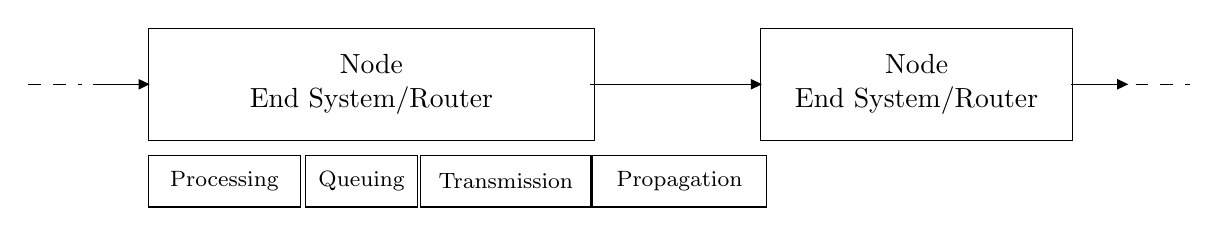
\begin{tikzpicture}[x=0.75pt,y=0.75pt,yscale=-1,xscale=1]
    %uncomment if require: \path (0,300); %set diagram left start at 0, and has height of 300
    
    %Straight Lines [id:da8558959419412624] 
    \draw    (136.5,161) -- (161,161) ;
    \draw [shift={(164,161)}, rotate = 180] [fill={rgb, 255:red, 0; green, 0; blue, 0 }  ][line width=0.08]  [draw opacity=0] (5.36,-2.57) -- (0,0) -- (5.36,2.57) -- cycle    ;
    %Straight Lines [id:da6707623693403982] 
    \draw  [dash pattern={on 4.5pt off 4.5pt}]  (105.5,161) -- (131.5,161) ;
    %Straight Lines [id:da7168530562511195] 
    \draw    (376.13,161) -- (456,161) ;
    \draw [shift={(459,161)}, rotate = 180] [fill={rgb, 255:red, 0; green, 0; blue, 0 }  ][line width=0.08]  [draw opacity=0] (5.36,-2.57) -- (0,0) -- (5.36,2.57) -- cycle    ;
    %Straight Lines [id:da9635909494137869] 
    \draw    (608,161) -- (632.5,161) ;
    \draw [shift={(635.5,161)}, rotate = 180] [fill={rgb, 255:red, 0; green, 0; blue, 0 }  ][line width=0.08]  [draw opacity=0] (5.36,-2.57) -- (0,0) -- (5.36,2.57) -- cycle    ;
    %Straight Lines [id:da58861118085922] 
    \draw  [dash pattern={on 4.5pt off 4.5pt}]  (639,161) -- (665,161) ;
    
    % Text Node
    \draw    (163.31,134) -- (378.31,134) -- (378.31,188) -- (163.31,188) -- cycle  ;
    \draw (270.81,161) node   [align=left] {\begin{minipage}[lt]{143.23pt}\setlength\topsep{0pt}
    \begin{center}
    Node\\End System/Router
    \end{center}
    
    \end{minipage}};
    % Text Node
    \draw    (458.5,134) -- (608.5,134) -- (608.5,188) -- (458.5,188) -- cycle  ;
    \draw (533.5,161) node   [align=left] {\begin{minipage}[lt]{99.28pt}\setlength\topsep{0pt}
    \begin{center}
    Node\\End System/Router
    \end{center}
    
    \end{minipage}};
    % Text Node
    \draw    (163.5,195.13) -- (236.5,195.13) -- (236.5,220.13) -- (163.5,220.13) -- cycle  ;
    \draw (200,207.63) node  [font=\footnotesize] [align=left] {\begin{minipage}[lt]{46.58pt}\setlength\topsep{0pt}
    \begin{center}
    Processing
    \end{center}
    
    \end{minipage}};
    % Text Node
    \draw    (239.13,195.13) -- (293.13,195.13) -- (293.13,220.13) -- (239.13,220.13) -- cycle  ;
    \draw (266.13,207.63) node  [font=\footnotesize] [align=left] {\begin{minipage}[lt]{33.83pt}\setlength\topsep{0pt}
    \begin{center}
    Queuing
    \end{center}
    
    \end{minipage}};
    % Text Node
    \draw    (294.63,195.13) -- (376.63,195.13) -- (376.63,220.13) -- (294.63,220.13) -- cycle  ;
    \draw (335.63,207.63) node  [font=\footnotesize] [align=left] {\begin{minipage}[lt]{52.87pt}\setlength\topsep{0pt}
    \begin{center}
    Transmission
    \end{center}
    
    \end{minipage}};
    % Text Node
    \draw    (377.25,195.13) -- (461.25,195.13) -- (461.25,220.13) -- (377.25,220.13) -- cycle  ;
    \draw (419.25,207.63) node  [font=\footnotesize] [align=left] {\begin{minipage}[lt]{54.06pt}\setlength\topsep{0pt}
    \begin{center}
    Propagation
    \end{center}
    
    \end{minipage}};
    
    
    \end{tikzpicture}
\caption{节点时延}
\end{figure}

\subsubsection{处理时延}

服务器需要先对分组进行一些检查和处理, 然后决定将该分组推入哪一条链路的传输队列中.
这一系列操作所占用的时间就是\textbf{处理时延} (processing delay),
记作 $d_\mathrm{proc}$.

\subsubsection{排队时延}

在当前节点通往后继节点的链路中, 有一个传输分组的队列 (或者说缓存). 任何需要通过
该链路传输的分组都必须先排队, 才能传输. 一般地, 某分组开始传输需要同时满足以下两个条件:
\begin{enumerate}[label={${\arabic*}^\circ$}, itemsep=0pt]
    \item 当前链路中没有其他分组正在传输;
    \item 当前队列中没有分组排在该分组前面,
\end{enumerate}
它的逆否命题是, 如果该链路当前正忙 (即正在传输其他的分组) 或者队列前面有其他的分组等待传输,
那么该分组只能老老实实地排队.

分组在传输队列上等待传输时所需要的时间就是\textbf{排队时延} (queuing delay),
记作 $d_\mathrm{queue}$,
某个分组的排队时延取决于队列前面正在等待传输的节点数量和链路的传输速度. 一般地说,
队列前方等待传输的分组数量是到达该队列的流量的强度和性质的函数.

排队时延是节点时延中最复杂, 也最有趣的成分. 与处理时延、传输时延和传播时延
不同的是, 排队时延对于不同的分组可能是不同的. 例如, 若干个分组同时到达空队列,
那么第一个分组没有排队时延, 可以直接传输, 而最后一个分组将要经受较大的排队时延. 因此
人们通常使用统计量——例如平均排队时延、排队时延的方差,
和排队时延超过某些特定值的概率——来度量、表征排队时延.

\subsubsection{传输时延}

将分组中的所有比特全部推入节点间的链路所需要的时间是\textbf{传输时延}
(transmission delay), 记作
$d_\mathrm{trans}$. 一般地, 速率为 $R \, \si{Mbps}$ 传输长度为 
$L \, \si{Mb}$ 的分组所需要的时间
\[ d_\mathrm{trans} = \dfrac{L}{R}. \]
在这里请一定要带着单位去计算, 注意 $\si{b}$ 和 $\si{B}$ 的区别, 此外,
在考虑数据传输的效率时, 我们一般是以 $10^3$ 作为基准来划定计数单位的\footnote{
    我们通常用 K, M, G, T 等符号来代表 $10^3$, $10^6$, $10^9$, $10^{12}, \cdots,$
    用 Ki, Mi, Gi, Ti 等符号来表示 $2^{10}, 2^{20}, 2^{30}, 2^{40}, \cdots$.
    这就是说, $1\si{KB} = 1000\si{B}$ 而 $1\si{KiB} = 1024\si{B}$.
}, 而不是
$2^{10}$. 这意味着, $1 \si{K} = 10^3$, $1 \si{M} = 10^6$,
$1 \si{T} = 10^9$, $1 \si{P} = 10^{12}$.
此外, 我们一般会把分组的长度 (即分组的数据量) 说成是分组的大小,
在本书中我们它们指的是一个意思, 都是在说这个分组里含有多少个 bit, 即含有多少个
二进制位.



\subsubsection{传播时延}

分组从链路的一端传播到另一端所需要的时间称为\textbf{传播时延} 
(propagation delay), 记作 $d_\mathrm{prop}$.
设链路的传播速率是 $s$, 链路两端之间的距离为 $d$, 那么传播时延
\[ d_\mathrm{prop} = \dfrac{d}{s}. \]
链路上的传播速率通常与链路本身有关, 也就是说这是一个由链路的物理性质所决定
的量, 数据传播采用的物理媒介不同, 传播速率也不同.

\vspace{1em}

在这里需要强调的是要注意传输时延和传播时延的区别. 传输时延是将分组从节点推入链路
所需要的时间, 它与分组长度和链路的传输速率有关, 与两节点之间的距离和链路的传播速率
无关; 而传播时延则是分组从链路的一端传播到另一端, 进入目的节点所需要的时间,
它与链路的传播速率和节点间的距离有关, 与节点到链路的传输速度和分组长度无关.
\begin{table}[H]
    \centering
    \caption{对比: 传输时延与传播时延}
    \begin{tabular}{cccp{0.4\textwidth}}
        \hline
        \textbf{时延类型} & \textbf{起始于……} & \textbf{终点是……} & \textbf{有关的影响因素} \\ 
        \hline
        传输时延 $d_\mathrm{trans}$ & 源节点 & 节点间的链路 & 节点-链路传输速率 $R$、分组长度 $L$ \\ 
        传播时延 $d_\mathrm{prop}$ & 节点间的链路 & 源节点 & 链路传播速率 $s$、节点间的距离 $d$ \\
        \hline
    \end{tabular}
\end{table}

如上文所述, 节点的总时延 (total nodal delay, 记作 $d_\mathrm{nodal}$)
就是处理时延、排队时延、传输时延和传播时延的累加,
因此我们有计算公式
\[ d_\mathrm{nodal} = d_\mathrm{proc}
+ d_\mathrm{queue} + d_\mathrm{trans} + d_\mathrm{prop}. \]
在不同的网络结构和传输场景中, 不同类别的时延所占据的比例是不同的. 例如, 同一个
大学内网中的两台计算机通信时, $d_\mathrm{prop}$ 可能微不足道, 但一台地面计算机
和轨道上的卫星通信时的 $d_\mathrm{prop}$ 可能就会占据 $d_\mathrm{nodal}$ 的
绝大部分了.

\subsection{流量强度 \quad 丢包}

\subsubsection{流量强度}

估计排队时延的一个常用的物理量是\textbf{流量强度} (traffic intensity),
它是单位时间内到达的数据量与节点向链路传输数据的速度的比值. 设单位时间内到达队列的
分组数量为 $a$, 它的单位是 $\si{pkt/s}$, 量纲是 $T^{-1}$, 它也被称为
分组到达队列的平均速率; 设节点向链路推入数据的传输速率为 $R$, 分组的长度为 $L$,
那么该节点-链路交界处的流量强度就是 $La/R$. 其中 $La$ 是单位时间内到达的数据量,
$R$ 是单位时间内被推入链路的数据量.

对于流量强度, 一般的规律是, {\kaishu 当流量强度接近于 $0$ 时, 队列中
要么分组到达的时间间隔很长, 要么分组的数据量很小, 所以传输队列中的分组不需要太长
的时间, 这时平均排队时延 $\bar{d}_\mathrm{queue}$ 将接近于 $0$; 但当流量强度
接近于 $1$, 平均排队时延将迅速增加, 这种情况下, 流量时延的少量扰动都将会导致平均
排队时延发生巨大的变化.}
总而言之, 我们有
\[ \bar{d}_\mathrm{queue} \to 0 \,  \text{for}  \, La/R \to 0, 
\quad \bar{d}_\mathrm{queue} \to +\infty \,  \text{for}  \, La/R \to 1. \]

\subsubsection{丢包}

\begin{figure}[H]
    \centering


\tikzset{every picture/.style={line width=0.75pt}} %set default line width to 0.75pt        

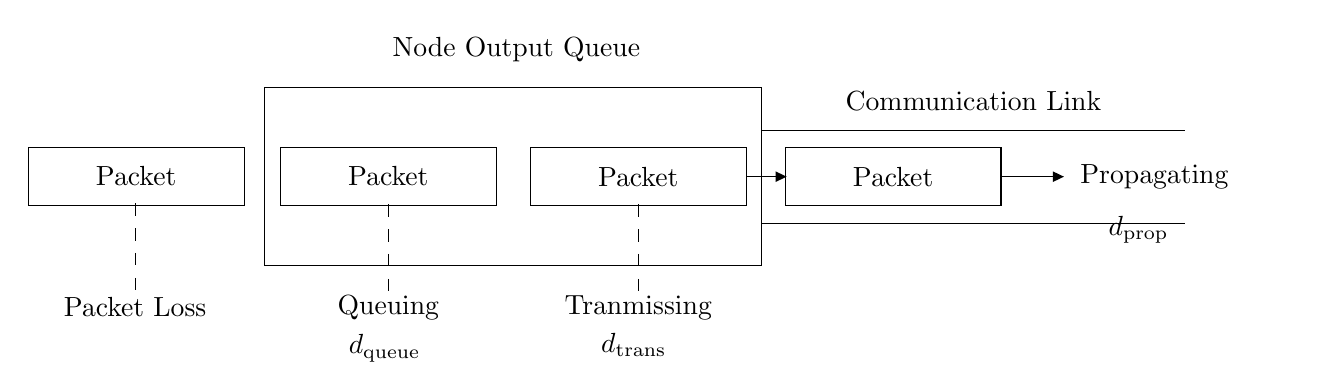
\begin{tikzpicture}[x=0.75pt,y=0.75pt,yscale=-1,xscale=1]
%uncomment if require: \path (0,300); %set diagram left start at 0, and has height of 300

%Flowchart: Process [id:dp13936489324248336] 
\draw   (152.5,112.5) -- (392,112.5) -- (392,198.25) -- (152.5,198.25) -- cycle ;
%Straight Lines [id:da7123310494862635] 
\draw    (392,133) -- (596,133) ;
%Straight Lines [id:da6800709939320764] 
\draw    (392,178) -- (596,178) ;
%Straight Lines [id:da6869250002399523] 
\draw    (506.8,155.35) -- (534.6,155.35) ;
\draw [shift={(537.6,155.35)}, rotate = 180] [fill={rgb, 255:red, 0; green, 0; blue, 0 }  ][line width=0.08]  [draw opacity=0] (5.36,-2.57) -- (0,0) -- (5.36,2.57) -- cycle    ;
%Straight Lines [id:da8804657167303325] 
\draw    (384.8,155.35) -- (401,155.35) ;
\draw [shift={(404,155.35)}, rotate = 180] [fill={rgb, 255:red, 0; green, 0; blue, 0 }  ][line width=0.08]  [draw opacity=0] (5.36,-2.57) -- (0,0) -- (5.36,2.57) -- cycle    ;
%Straight Lines [id:da5588264797649036] 
\draw  [dash pattern={on 4.5pt off 4.5pt}]  (332.5,168.6) -- (332.5,212.6) ;

%Straight Lines [id:da40973581115647206] 
\draw  [dash pattern={on 4.5pt off 4.5pt}]  (212.1,168.6) -- (212.1,212.6) ;

%Straight Lines [id:da028354607144250532] 
\draw  [dash pattern={on 4.5pt off 4.5pt}]  (90.1,168.1) -- (90.1,212.1) ;


% Text Node
\draw (273.75,93.93) node   [align=left] {\begin{minipage}[lt]{111.86pt}\setlength\topsep{0pt}
\begin{center}
Node Output Queue
\end{center}

\end{minipage}};
% Text Node
\draw (494,119) node   [align=left] {\begin{minipage}[lt]{107.98pt}\setlength\topsep{0pt}
\begin{center}
Communication Link
\end{center}

\end{minipage}};
% Text Node
\draw    (403.3,141.35) -- (507.3,141.35) -- (507.3,169.35) -- (403.3,169.35) -- cycle  ;
\draw (455.3,155.35) node   [align=left] {\begin{minipage}[lt]{68pt}\setlength\topsep{0pt}
\begin{center}
Packet
\end{center}

\end{minipage}};
% Text Node
\draw (581.2,155.35) node   [align=left] {\begin{minipage}[lt]{107.98pt}\setlength\topsep{0pt}
\begin{center}
Propagating
\end{center}

\end{minipage}};
% Text Node
\draw    (280.5,141.35) -- (384.5,141.35) -- (384.5,169.35) -- (280.5,169.35) -- cycle  ;
\draw (332.5,155.35) node   [align=left] {\begin{minipage}[lt]{68pt}\setlength\topsep{0pt}
\begin{center}
Packet
\end{center}

\end{minipage}};
% Text Node
\draw    (38.6,141.1) -- (142.6,141.1) -- (142.6,169.1) -- (38.6,169.1) -- cycle  ;
\draw (90.6,155.1) node   [align=left] {\begin{minipage}[lt]{68pt}\setlength\topsep{0pt}
\begin{center}
Packet
\end{center}

\end{minipage}};
% Text Node
\draw (90.1,218.05) node   [align=left] {\begin{minipage}[lt]{62.27pt}\setlength\topsep{0pt}
\begin{center}
Packet Loss
\end{center}

\end{minipage}};
% Text Node
\draw    (160.1,141.1) -- (264.1,141.1) -- (264.1,169.1) -- (160.1,169.1) -- cycle  ;
\draw (212.1,155.1) node   [align=left] {\begin{minipage}[lt]{68pt}\setlength\topsep{0pt}
\begin{center}
Packet
\end{center}

\end{minipage}};
% Text Node
\draw (212.1,218.55) node   [align=left] {\begin{minipage}[lt]{58.55pt}\setlength\topsep{0pt}
\begin{center}
Queuing
\end{center}

\end{minipage}};
% Text Node
\draw (191.8,230.2) node [anchor=north west][inner sep=0.75pt]    {$d_{\mathrm{queue}}$};
% Text Node
\draw (332.5,218.55) node   [align=left] {\begin{minipage}[lt]{58.55pt}\setlength\topsep{0pt}
\begin{center}
Tranmissing
\end{center}

\end{minipage}};
% Text Node
\draw (313.4,229.4) node [anchor=north west][inner sep=0.75pt]    {$d_{\mathrm{trans}}$};
% Text Node
\draw (557.9,173) node [anchor=north west][inner sep=0.75pt]    {$d_{\mathrm{prop}}$};


\end{tikzpicture}
\caption{丢包}
\end{figure}

节点输出队列能存储的数据量是有限的, 当节点输出队列已经装不下新到达的分组时,
由于没有地方存储这个分组, 路由器就将\textbf{丢弃} (drop) 这个分组,
分组丢包的比例将会随着流量强度的增加而增加. 丢包现象的存在, 说明我们不能仅仅依靠
时延来衡量数据传输的性能, 还要考虑丢包的问题.

\subsection{端到端时延}

接下来我们考虑从源端系统到目的端系统的时延, 不妨设从源端系统到目的端系统
之间有 $N-1$ 台路由器, 且此时网络是不拥塞的, 即忽略排队时延 $d_\mathrm{queue}$,
此外, 每台主机或路由器处理分组所需要的时间为 $d_\mathrm{proc}$,
每台主机或路由器的输出速率是 $R \si{bps}$, 每条链路的传播时延是
$d_\mathrm{prop}$.
那么把它们累加起来, 得到\textbf{端到端时延} (end-end delay):
\[ d_\mathrm{end-end} = N \left(
    d_\mathrm{proc} + d_\mathrm{trans} + d_\mathrm{prop}
\right). \]
根据传输时延的定义, 式中 $d_\mathrm{trans} = L/R$, 其中 $L$ 是以 $\si{b}$
计的分组长度, 即每个分组中 0/1 序列的位数.
于是, 端到端时延的一般形式为
\begin{equation}
    \label{equation: end-end delay}
    d_\mathrm{end-end} = N \left(
        d_\mathrm{proc} + \dfrac{L}{R} + d_\mathrm{prop}
    \right).
\end{equation}
如果各个分组的长度是不同的, 不同节点处的处理时延、平均排队时延和传输时延也是不同的,
不同节点之间的传播时延也不同的话, 那么 \ref{equation: end-end delay} 式
将会变成更一般化的形式:
\begin{equation}
    \label{equation: end-end delay_general}
    d_\mathrm{end-end}
    = \sum_{k=1}^{N}
    \sum_{i=1}^{n} \left( d_\mathrm{proc, i-1} 
    + \bar{d}_\mathrm{queue, i-1}
    + \dfrac{L_k}{R_{i-1}} + d_\mathrm{prop, (i-1,i)} \right),
\end{equation}
\ref{equation: end-end delay_general} 式中我们假设 $N$ 个分组
从源端系统 (节点索引为 $0$) 经历了 $n-1$ 个路由器
(这些路由器的节点索引分别为 $1,2,3,\cdots, n-1$) 最终到达了目的端系统 
(节点索引为 $n$),
第 $k$ 个分组的长度为 $L_k$, 第 $i$ 个节点的处理时延、平均排队时延和传输时延
分别为 $d_\mathrm{proc, i}$, $\bar{d}_\mathrm{queue, i}$ 和
$d_\mathrm{trans, i}$, 第 $i-1$ 个节点到第 $i$ 个节点的通信链路上的
传播时延为 $d_\mathrm{prop, (i-1,i)}$. 其中 $d_\mathrm{trans, i} =
L_k/R_i$, $R_i$ 表示第 $i$ 个节点将数据推入通往下一个节点的通信链路的传输速率.

\begin{example}
    假定在发送主机 $A$ 和接受主机 $B$ 间只有一台分组交换机 $S$, 
    发送主机和交换机间以及交换机
    和接受主机间的传输速率分别是 $R_1$ 和 $R_2$, 假设该交换机使用存储转发分组
    交换方式, 如果忽略排队时延、传播时延和处理时延 (这就是说, 我们只考虑传输时延),
    那么发送一个长度为 $L$ 的分组的
    端到端总时延 \[ d_\mathrm{end-end} = d_\mathrm{trans}(A, S)
    + d_\mathrm{trans}(S, A) = \dfrac{L}{R_1} + \dfrac{L}{R_2}. \]
\end{example}

\subsection{计算机网络中的吞吐量}

除了时延和丢包以外, 衡量计算机网络性能的另一个重要的指标是端到端吞吐量. 考虑从主机
A 到主机 B 跨越计算机网络传送一个大文件. 在任意给定的时刻, \textbf{瞬时吞吐量}
(instantaneous throughput) 是主机 B 接收到该文件的速率 (以 bps 计).
如果文件长度为 $T \si{bit}$, 而主机 B 花费了时间 $T \si{s}$ 去接收它,
则文件传送的\textbf{平均吞吐量} (average throughput) 是 $F/T \si{bps}$.

\begin{example}
    在如图 \ref{两链路网络} 所示的网络中, 服务器 S 和客户 C 通过一台路由器 R 相连, 要从服务器传送
    一个文件到客户, 其中, $R_\mathrm{s}$ 表示从服务器到路由器的链路的传输速率,
    $R_\mathrm{c}$ 则表示从路由器到客户的链路传输速率 (以 bps 计). 
    考虑这一情况下服务器到客户的网络吞吐量.
    \begin{figure}[H]
        \centering





        \tikzset{every picture/.style={line width=0.75pt}} %set default line width to 0.75pt        

        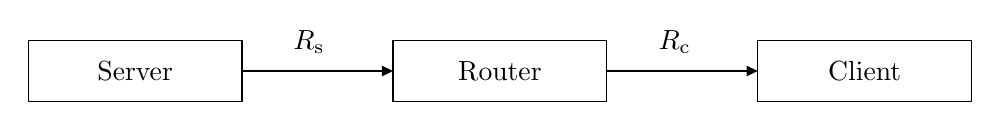
\begin{tikzpicture}[x=0.75pt,y=0.75pt,yscale=-1,xscale=1]
        %uncomment if require: \path (0,300); %set diagram left start at 0, and has height of 300
        
        %Straight Lines [id:da543368695511058] 
        \draw    (208.5,140.13) -- (278.25,140.13) ;
        \draw [shift={(281.25,140.13)}, rotate = 180] [fill={rgb, 255:red, 0; green, 0; blue, 0 }  ][line width=0.08]  [draw opacity=0] (5.36,-2.57) -- (0,0) -- (5.36,2.57) -- cycle    ;
        %Straight Lines [id:da7516766394891874] 
        \draw    (384.25,140.13) -- (454,140.13) ;
        \draw [shift={(457,140.13)}, rotate = 180] [fill={rgb, 255:red, 0; green, 0; blue, 0 }  ][line width=0.08]  [draw opacity=0] (5.36,-2.57) -- (0,0) -- (5.36,2.57) -- cycle    ;
        
        % Text Node
        \draw    (105.5,125.63) -- (208.5,125.63) -- (208.5,154.63) -- (105.5,154.63) -- cycle  ;
        \draw (157,140.13) node   [align=left] {\begin{minipage}[lt]{68pt}\setlength\topsep{0pt}
        \begin{center}
        Server
        \end{center}
        
        \end{minipage}};
        % Text Node
        \draw    (457,125.63) -- (560,125.63) -- (560,154.63) -- (457,154.63) -- cycle  ;
        \draw (508.5,140.13) node   [align=left] {\begin{minipage}[lt]{68pt}\setlength\topsep{0pt}
        \begin{center}
        Client
        \end{center}
        
        \end{minipage}};
        % Text Node
        \draw    (281.25,125.63) -- (384.25,125.63) -- (384.25,154.63) -- (281.25,154.63) -- cycle  ;
        \draw (332.75,140.13) node   [align=left] {\begin{minipage}[lt]{68pt}\setlength\topsep{0pt}
        \begin{center}
        Router
        \end{center}
        
        \end{minipage}};
        % Text Node
        \draw (232,119.52) node [anchor=north west][inner sep=0.75pt]    {$R_{\mathrm{s}}$};
        % Text Node
        \draw (408,119.52) node [anchor=north west][inner sep=0.75pt]    {$R_{\mathrm{c}}$};
        
        
        \end{tikzpicture}
        \caption{两链路网络}
        \label{两链路网络}
    \end{figure}
    在这一个网络中, 如果 $R_\mathrm{s} < R_\mathrm{c}$, 那么服务器中的数据
    将能够顺利地进入到链路中, 然后传输到路由器, 再经由第二条链路来到客户这一边,
    这时我们的吞吐量是 $R_\mathrm{s}$. 但如果 $R_\mathrm{c} < R_\mathrm{s}$,
    那么此时数据到达路由器的速度就会超出路由器把这些数据推入通信链路中的能力,
    这些数据会在路由器当中排队, 然后产生丢包, 这是我们所不愿意看到的.
    在计算机科学当中, {\kaishu 谁承担着数据传输的重任, 谁就有可能
    成为整个系统的瓶颈}, 这是一条普遍成立的一般性原理, 不光是计算机网络,
    在计算机组成原理或者其他学科当中, 你都有可能发现类似的规律.
    总而言之, 我们把这两条链路当中传输能力较弱的那一条成为\textbf{瓶颈链路}
    (bottleneck link), 在这个网络当中的吞吐量就是由瓶颈链路的传输能力所
    决定的, 这就是说, 对于如图 \ref{两链路网络} 所示的两链路网络而言,
    起吞吐量是 $\min \left\{ R_\mathrm{s}, R_\mathrm{c} \right\}$.
    
    于是我们现在可以对用户接收到完整的文件所需要的时间进行一个估计, 假设文件的大小
    (或者说长度) 是 $L \si{bit}$, 那么所需要的时间大概就是 $F/\min \left\{
        R_\mathrm{s}, R_\mathrm{c}
    \right\} \si{s}$.

    利用同样的原理, 我们可以把这一结论推广到含有链路更多的网络当中, 这时网络的吞吐率
    依然取决于其瓶颈链路的传输速率, 这就是说, 网络的吞吐率等于
    $\min \left\{ R_\mathrm{s}, R_1, R_2, \cdots, R_n \right\}$.
    \begin{figure}[H]
        \centering


\tikzset{every picture/.style={line width=0.75pt}} %set default line width to 0.75pt        

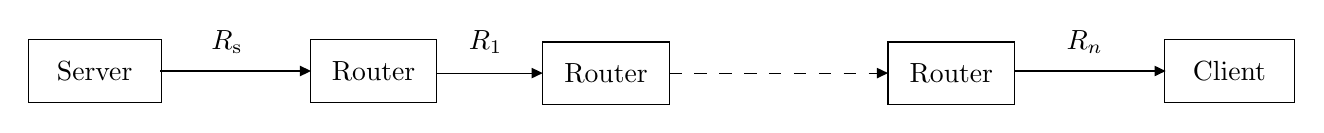
\begin{tikzpicture}[x=0.75pt,y=0.75pt,yscale=-1,xscale=1]
%uncomment if require: \path (0,300); %set diagram left start at 0, and has height of 300

%Straight Lines [id:da03182171179516091] 
\draw    (77.5,160.13) -- (147.25,160.13) ;
\draw [shift={(150.25,160.13)}, rotate = 180] [fill={rgb, 255:red, 0; green, 0; blue, 0 }  ][line width=0.08]  [draw opacity=0] (5.36,-2.57) -- (0,0) -- (5.36,2.57) -- cycle    ;
%Straight Lines [id:da2042401275622252] 
\draw    (489.25,160.13) -- (559,160.13) ;
\draw [shift={(562,160.13)}, rotate = 180] [fill={rgb, 255:red, 0; green, 0; blue, 0 }  ][line width=0.08]  [draw opacity=0] (5.36,-2.57) -- (0,0) -- (5.36,2.57) -- cycle    ;
%Straight Lines [id:da8297275105519664] 
\draw    (210.88,161.13) -- (258.88,161.13) ;
\draw [shift={(261.88,161.13)}, rotate = 180] [fill={rgb, 255:red, 0; green, 0; blue, 0 }  ][line width=0.08]  [draw opacity=0] (5.36,-2.57) -- (0,0) -- (5.36,2.57) -- cycle    ;
%Straight Lines [id:da85389589324296] 
\draw  [dash pattern={on 4.5pt off 4.5pt}]  (322.88,161.13) -- (425.25,161.13) ;
\draw [shift={(428.25,161.13)}, rotate = 180] [fill={rgb, 255:red, 0; green, 0; blue, 0 }  ][line width=0.08]  [draw opacity=0] (5.36,-2.57) -- (0,0) -- (5.36,2.57) -- cycle    ;

% Text Node
\draw    (14,145.13) -- (78,145.13) -- (78,175.13) -- (14,175.13) -- cycle  ;
\draw (46,160.13) node   [align=left] {\begin{minipage}[lt]{40.8pt}\setlength\topsep{0pt}
\begin{center}
Server
\end{center}

\end{minipage}};
% Text Node
\draw    (561.25,145.13) -- (624.25,145.13) -- (624.25,175.13) -- (561.25,175.13) -- cycle  ;
\draw (592.75,160.13) node   [align=left] {\begin{minipage}[lt]{39.78pt}\setlength\topsep{0pt}
\begin{center}
Client
\end{center}

\end{minipage}};
% Text Node
\draw    (149.88,145.13) -- (210.88,145.13) -- (210.88,175.13) -- (149.88,175.13) -- cycle  ;
\draw (180.38,160.13) node   [align=left] {\begin{minipage}[lt]{38.93pt}\setlength\topsep{0pt}
\begin{center}
Router
\end{center}

\end{minipage}};
% Text Node
\draw (101,139.52) node [anchor=north west][inner sep=0.75pt]    {$R_{\mathrm{s}}$};
% Text Node
\draw (513,139.52) node [anchor=north west][inner sep=0.75pt]    {$R_{n}$};
% Text Node
\draw    (428.25,146.13) -- (489.25,146.13) -- (489.25,176.13) -- (428.25,176.13) -- cycle  ;
\draw (458.75,161.13) node   [align=left] {\begin{minipage}[lt]{38.93pt}\setlength\topsep{0pt}
\begin{center}
Router
\end{center}

\end{minipage}};
% Text Node
\draw    (261.88,146.13) -- (322.88,146.13) -- (322.88,176.13) -- (261.88,176.13) -- cycle  ;
\draw (292.38,161.13) node   [align=left] {\begin{minipage}[lt]{38.93pt}\setlength\topsep{0pt}
\begin{center}
Router
\end{center}

\end{minipage}};
% Text Node
\draw (225,139.52) node [anchor=north west][inner sep=0.75pt]    {$R_{1}$};


\end{tikzpicture}
    \end{figure}
\end{example}

\begin{example}
    现在考虑若干个用户通过同一个网络核心向若干个服务器请求数据.
    这时对于一个 Server-Client 端到端连接来说, 要传输的数据会受到
    网络核心中其他连接传输数据的干扰. 这时, 网络的吞吐量就不仅取决于沿着路径的
    传输速率的大小了, 还取决于网络中的干扰流量. 事实上, 如果许多其他的数据流也通过
    这个网络核心在流动, 那么这个网络核心也有可能会成为整个连接当中的瓶颈 (尽管在一般情况下,
    网络核心就像一根粗大的管子, 影响吞吐率的往往是网络边缘).
    \begin{figure}[H]
        \centering


\tikzset{every picture/.style={line width=0.75pt}} %set default line width to 0.75pt        

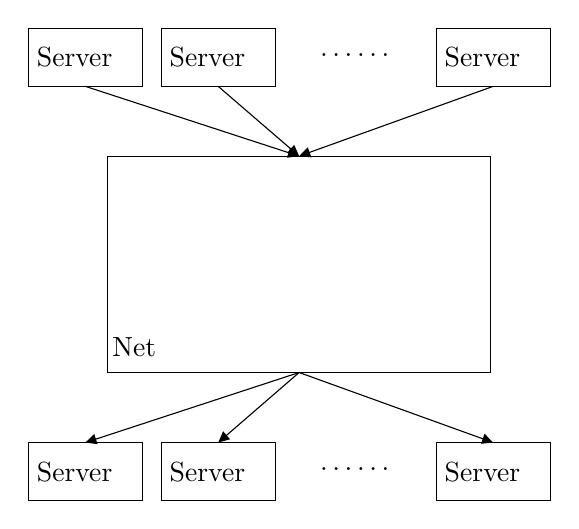
\begin{tikzpicture}[x=0.75pt,y=0.75pt,yscale=-1,xscale=1]
%uncomment if require: \path (0,300); %set diagram left start at 0, and has height of 300

%Shape: Rectangle [id:dp6268850326190047] 
\draw   (176,88.5) -- (360.5,88.5) -- (360.5,192.75) -- (176,192.75) -- cycle ;
%Straight Lines [id:da7100920200856897] 
\draw    (165.25,54.88) -- (265.4,87.57) ;
\draw [shift={(268.25,88.5)}, rotate = 198.08] [fill={rgb, 255:red, 0; green, 0; blue, 0 }  ][line width=0.08]  [draw opacity=0] (5.36,-2.57) -- (0,0) -- (5.36,2.57) -- cycle    ;
%Straight Lines [id:da2981299356553365] 
\draw    (229.25,54.88) -- (265.98,86.54) ;
\draw [shift={(268.25,88.5)}, rotate = 220.77] [fill={rgb, 255:red, 0; green, 0; blue, 0 }  ][line width=0.08]  [draw opacity=0] (5.36,-2.57) -- (0,0) -- (5.36,2.57) -- cycle    ;
%Straight Lines [id:da3127825640800619] 
\draw    (361.75,54.88) -- (271.07,87.48) ;
\draw [shift={(268.25,88.5)}, rotate = 340.22] [fill={rgb, 255:red, 0; green, 0; blue, 0 }  ][line width=0.08]  [draw opacity=0] (5.36,-2.57) -- (0,0) -- (5.36,2.57) -- cycle    ;
%Straight Lines [id:da4016812223274324] 
\draw    (168.1,225.57) -- (268.25,192.75) ;
\draw [shift={(165.25,226.5)}, rotate = 341.86] [fill={rgb, 255:red, 0; green, 0; blue, 0 }  ][line width=0.08]  [draw opacity=0] (5.36,-2.57) -- (0,0) -- (5.36,2.57) -- cycle    ;
%Straight Lines [id:da48100265837676637] 
\draw    (231.52,224.54) -- (268.25,192.75) ;
\draw [shift={(229.25,226.5)}, rotate = 319.13] [fill={rgb, 255:red, 0; green, 0; blue, 0 }  ][line width=0.08]  [draw opacity=0] (5.36,-2.57) -- (0,0) -- (5.36,2.57) -- cycle    ;
%Straight Lines [id:da6198566001075859] 
\draw    (358.93,225.48) -- (268.25,192.75) ;
\draw [shift={(361.75,226.5)}, rotate = 199.85] [fill={rgb, 255:red, 0; green, 0; blue, 0 }  ][line width=0.08]  [draw opacity=0] (5.36,-2.57) -- (0,0) -- (5.36,2.57) -- cycle    ;

% Text Node
\draw    (137.75,26.88) -- (192.75,26.88) -- (192.75,54.88) -- (137.75,54.88) -- cycle  ;
\draw (165.25,40.88) node   [align=left] {\begin{minipage}[lt]{35.02pt}\setlength\topsep{0pt}
Server
\end{minipage}};
% Text Node
\draw    (201.75,26.88) -- (256.75,26.88) -- (256.75,54.88) -- (201.75,54.88) -- cycle  ;
\draw (229.25,40.88) node   [align=left] {\begin{minipage}[lt]{35.02pt}\setlength\topsep{0pt}
Server
\end{minipage}};
% Text Node
\draw    (334.25,26.88) -- (389.25,26.88) -- (389.25,54.88) -- (334.25,54.88) -- cycle  ;
\draw (361.75,40.88) node   [align=left] {\begin{minipage}[lt]{35.02pt}\setlength\topsep{0pt}
Server
\end{minipage}};
% Text Node
\draw (301.25,40.88) node   [align=left] {\begin{minipage}[lt]{34.34pt}\setlength\topsep{0pt}
……
\end{minipage}};
% Text Node
\draw (199.75,180.25) node   [align=left] {\begin{minipage}[lt]{32.3pt}\setlength\topsep{0pt}
Net
\end{minipage}};
% Text Node
\draw    (137.75,226.5) -- (192.75,226.5) -- (192.75,254.5) -- (137.75,254.5) -- cycle  ;
\draw (165.25,240.5) node   [align=left] {\begin{minipage}[lt]{35.02pt}\setlength\topsep{0pt}
Server
\end{minipage}};
% Text Node
\draw    (201.75,226.5) -- (256.75,226.5) -- (256.75,254.5) -- (201.75,254.5) -- cycle  ;
\draw (229.25,240.5) node   [align=left] {\begin{minipage}[lt]{35.02pt}\setlength\topsep{0pt}
Server
\end{minipage}};
% Text Node
\draw    (334.25,226.5) -- (389.25,226.5) -- (389.25,254.5) -- (334.25,254.5) -- cycle  ;
\draw (361.75,240.5) node   [align=left] {\begin{minipage}[lt]{35.02pt}\setlength\topsep{0pt}
Server
\end{minipage}};
% Text Node
\draw (301.25,240.5) node   [align=left] {\begin{minipage}[lt]{34.34pt}\setlength\topsep{0pt}
……
\end{minipage}};


\end{tikzpicture}
    \end{figure}
\end{example}

\section{协议层次及其服务模型}

\subsection{分层的体系结构}

% \subsubsection{分层的好处}
% \subsubsection{因特网的协议栈}

\begin{figure}[H]
    \centering
    

\tikzset{every picture/.style={line width=0.75pt}} %set default line width to 0.75pt        

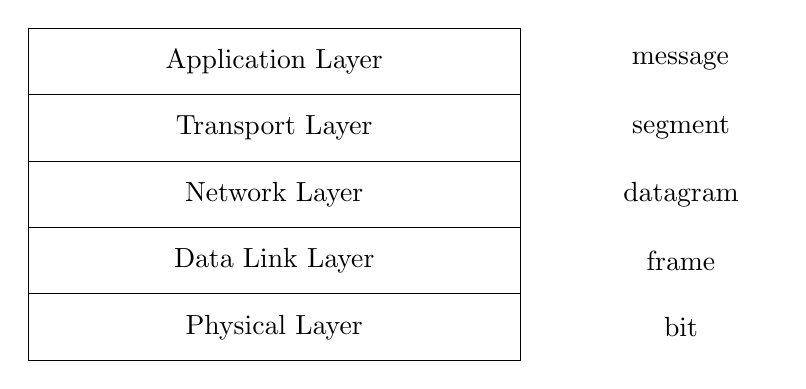
\begin{tikzpicture}[x=0.75pt,y=0.75pt,yscale=-1,xscale=1]
%uncomment if require: \path (0,300); %set diagram left start at 0, and has height of 300


% Text Node
\draw    (153,75.75) -- (390,75.75) -- (390,107.75) -- (153,107.75) -- cycle  ;
\draw (271.5,91.75) node   [align=left] {\begin{minipage}[lt]{158.44pt}\setlength\topsep{0pt}
\begin{center}
Application Layer
\end{center}

\end{minipage}};
% Text Node
\draw    (153,107.75) -- (390,107.75) -- (390,139.75) -- (153,139.75) -- cycle  ;
\draw (271.5,123.75) node   [align=left] {\begin{minipage}[lt]{158.44pt}\setlength\topsep{0pt}
\begin{center}
Transport Layer
\end{center}

\end{minipage}};
% Text Node
\draw    (153,139.75) -- (390,139.75) -- (390,171.75) -- (153,171.75) -- cycle  ;
\draw (271.5,155.75) node   [align=left] {\begin{minipage}[lt]{158.44pt}\setlength\topsep{0pt}
\begin{center}
Network Layer
\end{center}

\end{minipage}};
% Text Node
\draw    (153,171.75) -- (390,171.75) -- (390,203.75) -- (153,203.75) -- cycle  ;
\draw (271.5,187.75) node   [align=left] {\begin{minipage}[lt]{158.44pt}\setlength\topsep{0pt}
\begin{center}
Data Link Layer
\end{center}

\end{minipage}};
% Text Node
\draw    (153,203.75) -- (390,203.75) -- (390,235.75) -- (153,235.75) -- cycle  ;
\draw (271.5,219.75) node   [align=left] {\begin{minipage}[lt]{158.44pt}\setlength\topsep{0pt}
\begin{center}
Physical Layer
\end{center}

\end{minipage}};
% Text Node
\draw (467.25,91.75) node   [align=left] {\begin{minipage}[lt]{63.58pt}\setlength\topsep{0pt}
\begin{center}
message
\end{center}

\end{minipage}};
% Text Node
\draw (467.5,123.75) node   [align=left] {\begin{minipage}[lt]{63.58pt}\setlength\topsep{0pt}
\begin{center}
segment
\end{center}

\end{minipage}};
% Text Node
\draw (467.5,155.75) node   [align=left] {\begin{minipage}[lt]{63.58pt}\setlength\topsep{0pt}
\begin{center}
datagram
\end{center}

\end{minipage}};
% Text Node
\draw (467.5,187.75) node   [align=left] {\begin{minipage}[lt]{63.58pt}\setlength\topsep{0pt}
\begin{center}
frame
\end{center}

\end{minipage}};
% Text Node
\draw (467.5,219.75) node   [align=left] {\begin{minipage}[lt]{63.58pt}\setlength\topsep{0pt}
\begin{center}
bit
\end{center}

\end{minipage}};


\end{tikzpicture}
\caption{因特网的协议栈}
\label{因特网的协议栈}
\end{figure}

各个层次的所有协议被称为\textbf{协议栈} (protocol stack),
如图 \ref{因特网的协议栈} 所示, 因特网的协议栈由 5 个层次组成: 应用层、
传输层、网络层、链路层、物理层. 
\begin{enumerate}[label={$\left.\mathrm{\alph*}\right)$}, itemsep=0pt]
    \item \textbf{应用层} (Application Layer):
    应用层是网络应用程序及其应用层协议所在的层次, 它分布于多个端系统上,
    一个端系统中的网络应用程序使用协议与另一个端系统中的网络应用程序交换
    信息分组, 这种信息分组成为\textbf{报文} (message), 用 M 表示. 应用层提供了
    用户与网络服务之间的接口, 使用户能够访问各种网络应用和网络服务.
    \item \textbf{运输层} (Transport Layer):
    运输层收取应用层报文分组并附上运输层首部信息 $\mathrm{H}_\mathrm{t}$,
    一同构成\textbf{运输层报文段} (transport-layer segment), 
    注意一个大报文分组可能会被划分为多个应用层报文段分组 (下列各层同理, 这意味着在接收端
    必须从连续的报文段中重新把大报文给 “拼装” 出来.),
    然后在网络应用程序端点之间传送, 到达目的端系统后, 需要将报文上交给应用层.
    \begin{itemize}[itemsep=0pt]
        \item 允许接收端运输层向上向适当的应用程序交付报文的信息;
        \item 差错检测位信息: 该信息让接收端能够判断报文中的比特是否在途中已被改变;
    \end{itemize}
    \item \textbf{网络层} (Network Layer): 网络层负责传输路线的选取,
    将源端系统和目的端系统地址等附加信息 $H_n$ 封装到运输层报文段分组中, 得到\textbf{网络层数据报}
    (network-layer datagram), 然后传输给链路层.
    \item \textbf{链路层} (Data Link Layer): 链路层负责在临近的网络节点之间传输数据,
    链路层在接收到网络层下派的数据报分组后, 在其分组上附加
    链路层首部信息 $\mathrm{H_l}$ 并生成\textbf{链路层帧} (data-link-layer frame),
    然后交付到物理层实现在链路上的传输.
    \item \textbf{物理层} (Physical Layer): 将帧中的\textbf{比特} (bit,
    即一位 0/1 序列) 以比特流的形式从链路的一个端点移动到另一个端点, 物理层决定并保证了
    网络物理连接的特性、拓扑结构, 定义了数据传输的物理规范.
\end{enumerate}
在因特网的协议栈中, 下层是上层的实现, 上层使用下层提供的服务来实现本层次的功能.
下层\textbf{封装} (encapsulation) 上层分组并附加自己的首部信息,
然后传递给在再下一层处理.

在每一层, 一个分组具有两种类型的字段, 分别是\textbf{首部字段} (head field) 和
\textbf{有效载荷字段} (payload field), 有效载荷通常来自上一层分组.



% \subsection{封装}

数据从发送端系统 (Source) 的协议栈向下, 沿着中间的链路层交换机 (Data Link Layer Switch) 
和路由器 (Router) 的协议栈上上下下, 然后向上到达接收端系统 (Destination) 的协议栈.

\begin{figure}[H]
    \centering


\tikzset{every picture/.style={line width=0.75pt}} %set default line width to 0.75pt        

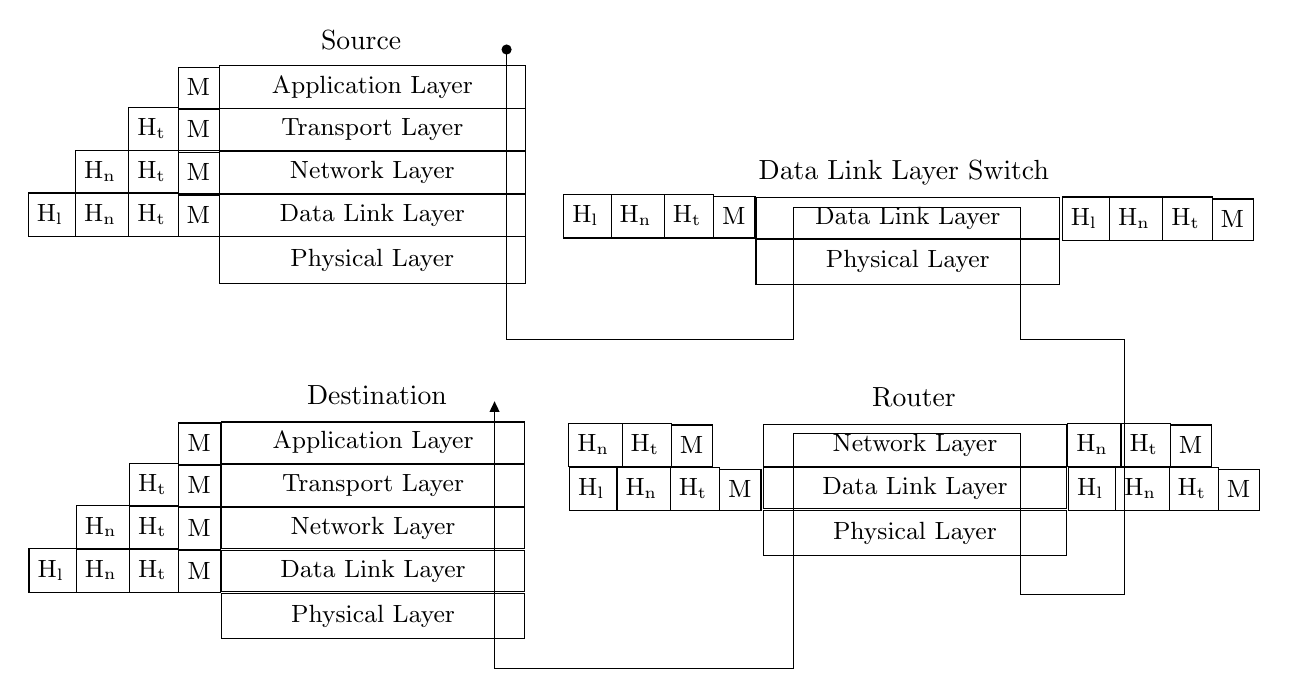
\begin{tikzpicture}[x=0.75pt,y=0.75pt,yscale=-0.95,xscale=0.95]
%uncomment if require: \path (0,370); %set diagram left start at 0, and has height of 370



%Shape: Boxed Line [id:dp18001549214427603] 
\draw    (271.4,11.8) -- (271.4,159) -- (417,159) -- (417,91.8) -- (532.2,91.8) -- (532.2,159) -- (585,159) -- (585,288.2) -- (532.2,288.2) -- (532.2,206.6) -- (417,206.6) -- (417,325.91) -- (265.3,325.91) -- (265.3,193.2) ;
\draw [shift={(265.3,190.2)}, rotate = 90] [fill={rgb, 255:red, 0; green, 0; blue, 0 }  ][line width=0.08]  [draw opacity=0] (5.36,-2.57) -- (0,0) -- (5.36,2.57) -- cycle    ;
\draw [shift={(271.4,11.8)}, rotate = 90] [color={rgb, 255:red, 0; green, 0; blue, 0 }  ][fill={rgb, 255:red, 0; green, 0; blue, 0 }  ][line width=0.75]      (0, 0) circle [x radius= 2.01, y radius= 2.01]   ;







% Text Node
\draw    (125.8,19.81) -- (280.8,19.81) -- (280.8,41.81) -- (125.8,41.81) -- cycle  ;
\draw (203.3,30.81) node  [font=\small] [align=left] {\begin{minipage}[lt]{102.4pt}\setlength\topsep{0pt}
\begin{center}
Application Layer
\end{center}

\end{minipage}};
% Text Node
\draw    (125.8,41.49) -- (280.8,41.49) -- (280.8,63.49) -- (125.8,63.49) -- cycle  ;
\draw (203.3,52.49) node  [font=\small] [align=left] {\begin{minipage}[lt]{102.4pt}\setlength\topsep{0pt}
\begin{center}
Transport Layer
\end{center}

\end{minipage}};
% Text Node
\draw    (125.8,63.17) -- (280.8,63.17) -- (280.8,85.17) -- (125.8,85.17) -- cycle  ;
\draw (203.3,74.17) node  [font=\small] [align=left] {\begin{minipage}[lt]{102.4pt}\setlength\topsep{0pt}
\begin{center}
Network Layer
\end{center}

\end{minipage}};
% Text Node
\draw    (125.8,84.85) -- (280.8,84.85) -- (280.8,106.85) -- (125.8,106.85) -- cycle  ;
\draw (203.3,95.85) node  [font=\small] [align=left] {\begin{minipage}[lt]{102.4pt}\setlength\topsep{0pt}
\begin{center}
Data Link Layer
\end{center}

\end{minipage}};
% Text Node
\draw    (125.8,106.59) -- (280.8,106.59) -- (280.8,130.59) -- (125.8,130.59) -- cycle  ;
\draw (203.3,118.59) node  [font=\small] [align=left] {\begin{minipage}[lt]{102.4pt}\setlength\topsep{0pt}
\begin{center}
Physical Layer
\end{center}

\end{minipage}};
% Text Node
\draw (176,1) node [anchor=north west][inner sep=0.75pt]   [align=left] {Source};
% Text Node
\draw    (79.8,41.17) -- (104.8,41.17) -- (104.8,63.17) -- (79.8,63.17) -- cycle  ;
\draw (82.8,45.57) node [anchor=north west][inner sep=0.75pt]  [font=\small]  {$\mathrm{H}_{\mathrm{t}}$};
% Text Node
\draw    (104.8,20.81) -- (125.8,20.81) -- (125.8,41.81) -- (104.8,41.81) -- cycle  ;
\draw (107.8,25.21) node [anchor=north west][inner sep=0.75pt]  [font=\small]  {$\mathrm{M}$};
% Text Node
\draw    (104.8,42.17) -- (125.8,42.17) -- (125.8,63.17) -- (104.8,63.17) -- cycle  ;
\draw (107.8,46.57) node [anchor=north west][inner sep=0.75pt]  [font=\small]  {$\mathrm{M}$};
% Text Node
\draw    (79.8,84.59) -- (104.8,84.59) -- (104.8,106.59) -- (79.8,106.59) -- cycle  ;
\draw (82.8,88.99) node [anchor=north west][inner sep=0.75pt]  [font=\small]  {$\mathrm{H}_{\mathrm{t}}$};
% Text Node
\draw    (104.8,85.59) -- (125.8,85.59) -- (125.8,106.59) -- (104.8,106.59) -- cycle  ;
\draw (107.8,89.99) node [anchor=north west][inner sep=0.75pt]  [font=\small]  {$\mathrm{M}$};
% Text Node
\draw    (52.8,84.59) -- (79.8,84.59) -- (79.8,106.59) -- (52.8,106.59) -- cycle  ;
\draw (55.8,88.99) node [anchor=north west][inner sep=0.75pt]  [font=\small]  {$\mathrm{H}_{\mathrm{n}}$};
% Text Node
\draw    (28.8,84.59) -- (52.8,84.59) -- (52.8,106.59) -- (28.8,106.59) -- cycle  ;
\draw (31.8,88.99) node [anchor=north west][inner sep=0.75pt]  [font=\small]  {$\mathrm{H}_{\mathrm{l}}$};
% Text Node
\draw    (397.9,86.89) -- (551.9,86.89) -- (551.9,107.89) -- (397.9,107.89) -- cycle  ;
\draw (474.9,97.39) node  [font=\small] [align=left] {\begin{minipage}[lt]{102.4pt}\setlength\topsep{0pt}
\begin{center}
Data Link Layer
\end{center}

\end{minipage}};
% Text Node
\draw    (397.9,107.89) -- (551.9,107.89) -- (551.9,130.89) -- (397.9,130.89) -- cycle  ;
\draw (474.9,119.39) node  [font=\small] [align=left] {\begin{minipage}[lt]{102.4pt}\setlength\topsep{0pt}
\begin{center}
Physical Layer
\end{center}

\end{minipage}};
% Text Node
\draw (397.9,66.89) node [anchor=north west][inner sep=0.75pt]   [align=left] {Data Link Layer Switch};
% Text Node
\draw    (351.4,85.39) -- (376.4,85.39) -- (376.4,107.39) -- (351.4,107.39) -- cycle  ;
\draw (354.4,89.79) node [anchor=north west][inner sep=0.75pt]  [font=\small]  {$\mathrm{H}_{\mathrm{t}}$};
% Text Node
\draw    (376.4,86.39) -- (397.4,86.39) -- (397.4,107.39) -- (376.4,107.39) -- cycle  ;
\draw (379.4,90.79) node [anchor=north west][inner sep=0.75pt]  [font=\small]  {$\mathrm{M}$};
% Text Node
\draw    (324.4,85.39) -- (351.4,85.39) -- (351.4,107.39) -- (324.4,107.39) -- cycle  ;
\draw (327.4,89.79) node [anchor=north west][inner sep=0.75pt]  [font=\small]  {$\mathrm{H}_{\mathrm{n}}$};
% Text Node
\draw    (300.4,85.39) -- (324.4,85.39) -- (324.4,107.39) -- (300.4,107.39) -- cycle  ;
\draw (303.4,89.79) node [anchor=north west][inner sep=0.75pt]  [font=\small]  {$\mathrm{H}_{\mathrm{l}}$};
% Text Node
\draw    (553.2,86.59) -- (577.2,86.59) -- (577.2,108.59) -- (553.2,108.59) -- cycle  ;
\draw (556.2,90.99) node [anchor=north west][inner sep=0.75pt]  [font=\small]  {$\mathrm{H}_{\mathrm{l}}$};
% Text Node
\draw    (577.2,86.59) -- (604.2,86.59) -- (604.2,108.59) -- (577.2,108.59) -- cycle  ;
\draw (580.2,90.99) node [anchor=north west][inner sep=0.75pt]  [font=\small]  {$\mathrm{H}_{\mathrm{n}}$};
% Text Node
\draw    (629.2,87.59) -- (650.2,87.59) -- (650.2,108.59) -- (629.2,108.59) -- cycle  ;
\draw (632.2,91.99) node [anchor=north west][inner sep=0.75pt]  [font=\small]  {$\mathrm{M}$};
% Text Node
\draw    (604.2,86.59) -- (629.2,86.59) -- (629.2,108.59) -- (604.2,108.59) -- cycle  ;
\draw (607.2,90.99) node [anchor=north west][inner sep=0.75pt]  [font=\small]  {$\mathrm{H}_{\mathrm{t}}$};
% Text Node
\draw    (401.5,202.07) -- (555.5,202.07) -- (555.5,223.07) -- (401.5,223.07) -- cycle  ;
\draw (478.5,212.57) node  [font=\small] [align=left] {\begin{minipage}[lt]{102.4pt}\setlength\topsep{0pt}
\begin{center}
Network Layer
\end{center}

\end{minipage}};
% Text Node
\draw    (401.5,223.75) -- (555.5,223.75) -- (555.5,244.75) -- (401.5,244.75) -- cycle  ;
\draw (478.5,234.25) node  [font=\small] [align=left] {\begin{minipage}[lt]{102.4pt}\setlength\topsep{0pt}
\begin{center}
Data Link Layer
\end{center}

\end{minipage}};
% Text Node
\draw    (401.5,245.49) -- (555.5,245.49) -- (555.5,268.49) -- (401.5,268.49) -- cycle  ;
\draw (478.5,256.99) node  [font=\small] [align=left] {\begin{minipage}[lt]{102.4pt}\setlength\topsep{0pt}
\begin{center}
Physical Layer
\end{center}

\end{minipage}};
% Text Node
\draw (455.5,182.09) node [anchor=north west][inner sep=0.75pt]   [align=left] {Router};
% Text Node
\draw    (556.4,223.79) -- (580.4,223.79) -- (580.4,245.79) -- (556.4,245.79) -- cycle  ;
\draw (559.4,228.19) node [anchor=north west][inner sep=0.75pt]  [font=\small]  {$\mathrm{H}_{\mathrm{l}}$};
% Text Node
\draw    (580.4,223.79) -- (607.4,223.79) -- (607.4,245.79) -- (580.4,245.79) -- cycle  ;
\draw (583.4,228.19) node [anchor=north west][inner sep=0.75pt]  [font=\small]  {$\mathrm{H}_{\mathrm{n}}$};
% Text Node
\draw    (632.4,224.79) -- (653.4,224.79) -- (653.4,245.79) -- (632.4,245.79) -- cycle  ;
\draw (635.4,229.19) node [anchor=north west][inner sep=0.75pt]  [font=\small]  {$\mathrm{M}$};
% Text Node
\draw    (607.4,223.79) -- (632.4,223.79) -- (632.4,245.79) -- (607.4,245.79) -- cycle  ;
\draw (610.4,228.19) node [anchor=north west][inner sep=0.75pt]  [font=\small]  {$\mathrm{H}_{\mathrm{t}}$};
% Text Node
\draw    (79.8,62.85) -- (104.8,62.85) -- (104.8,84.85) -- (79.8,84.85) -- cycle  ;
\draw (82.8,67.25) node [anchor=north west][inner sep=0.75pt]  [font=\small]  {$\mathrm{H}_{\mathrm{t}}$};
% Text Node
\draw    (104.8,63.85) -- (125.8,63.85) -- (125.8,84.85) -- (104.8,84.85) -- cycle  ;
\draw (107.8,68.25) node [anchor=north west][inner sep=0.75pt]  [font=\small]  {$\mathrm{M}$};
% Text Node
\draw    (52.8,62.85) -- (79.8,62.85) -- (79.8,84.85) -- (52.8,84.85) -- cycle  ;
\draw (55.8,67.25) node [anchor=north west][inner sep=0.75pt]  [font=\small]  {$\mathrm{H}_{\mathrm{n}}$};
% Text Node
\draw    (556,201.25) -- (583,201.25) -- (583,223.25) -- (556,223.25) -- cycle  ;
\draw (559,205.65) node [anchor=north west][inner sep=0.75pt]  [font=\small]  {$\mathrm{H}_{\mathrm{n}}$};
% Text Node
\draw    (608,202.25) -- (629,202.25) -- (629,223.25) -- (608,223.25) -- cycle  ;
\draw (611,206.65) node [anchor=north west][inner sep=0.75pt]  [font=\small]  {$\mathrm{M}$};
% Text Node
\draw    (583,201.25) -- (608,201.25) -- (608,223.25) -- (583,223.25) -- cycle  ;
\draw (586,205.65) node [anchor=north west][inner sep=0.75pt]  [font=\small]  {$\mathrm{H}_{\mathrm{t}}$};
% Text Node
\draw    (303,201.25) -- (330,201.25) -- (330,223.25) -- (303,223.25) -- cycle  ;
\draw (306,205.65) node [anchor=north west][inner sep=0.75pt]  [font=\small]  {$\mathrm{H}_{\mathrm{n}}$};
% Text Node
\draw    (355,202.25) -- (376,202.25) -- (376,223.25) -- (355,223.25) -- cycle  ;
\draw (358,206.65) node [anchor=north west][inner sep=0.75pt]  [font=\small]  {$\mathrm{M}$};
% Text Node
\draw    (330,201.25) -- (355,201.25) -- (355,223.25) -- (330,223.25) -- cycle  ;
\draw (333,205.65) node [anchor=north west][inner sep=0.75pt]  [font=\small]  {$\mathrm{H}_{\mathrm{t}}$};
% Text Node
\draw    (303.4,223.79) -- (327.4,223.79) -- (327.4,245.79) -- (303.4,245.79) -- cycle  ;
\draw (306.4,228.19) node [anchor=north west][inner sep=0.75pt]  [font=\small]  {$\mathrm{H}_{\mathrm{l}}$};
% Text Node
\draw    (327.4,223.79) -- (354.4,223.79) -- (354.4,245.79) -- (327.4,245.79) -- cycle  ;
\draw (330.4,228.19) node [anchor=north west][inner sep=0.75pt]  [font=\small]  {$\mathrm{H}_{\mathrm{n}}$};
% Text Node
\draw    (379.4,224.79) -- (400.4,224.79) -- (400.4,245.79) -- (379.4,245.79) -- cycle  ;
\draw (382.4,229.19) node [anchor=north west][inner sep=0.75pt]  [font=\small]  {$\mathrm{M}$};
% Text Node
\draw    (354.4,223.79) -- (379.4,223.79) -- (379.4,245.79) -- (354.4,245.79) -- cycle  ;
\draw (357.4,228.19) node [anchor=north west][inner sep=0.75pt]  [font=\small]  {$\mathrm{H}_{\mathrm{t}}$};
% Text Node
\draw    (126.7,200.71) -- (280.7,200.71) -- (280.7,221.71) -- (126.7,221.71) -- cycle  ;
\draw (203.7,211.21) node  [font=\small] [align=left] {\begin{minipage}[lt]{102.4pt}\setlength\topsep{0pt}
\begin{center}
Application Layer
\end{center}

\end{minipage}};
% Text Node
\draw    (126.7,222.39) -- (280.7,222.39) -- (280.7,243.39) -- (126.7,243.39) -- cycle  ;
\draw (203.7,232.89) node  [font=\small] [align=left] {\begin{minipage}[lt]{102.4pt}\setlength\topsep{0pt}
\begin{center}
Transport Layer
\end{center}

\end{minipage}};
% Text Node
\draw    (126.7,244.07) -- (280.7,244.07) -- (280.7,265.07) -- (126.7,265.07) -- cycle  ;
\draw (203.7,254.57) node  [font=\small] [align=left] {\begin{minipage}[lt]{102.4pt}\setlength\topsep{0pt}
\begin{center}
Network Layer
\end{center}

\end{minipage}};
% Text Node
\draw    (126.7,265.75) -- (280.7,265.75) -- (280.7,286.75) -- (126.7,286.75) -- cycle  ;
\draw (203.7,276.25) node  [font=\small] [align=left] {\begin{minipage}[lt]{102.4pt}\setlength\topsep{0pt}
\begin{center}
Data Link Layer
\end{center}

\end{minipage}};
% Text Node
\draw    (126.7,287.49) -- (280.7,287.49) -- (280.7,310.49) -- (126.7,310.49) -- cycle  ;
\draw (203.7,298.99) node  [font=\small] [align=left] {\begin{minipage}[lt]{102.4pt}\setlength\topsep{0pt}
\begin{center}
Physical Layer
\end{center}

\end{minipage}};
% Text Node
\draw (168.9,180.71) node [anchor=north west][inner sep=0.75pt]   [align=left] {Destination};
% Text Node
\draw    (80.2,221.57) -- (105.2,221.57) -- (105.2,243.57) -- (80.2,243.57) -- cycle  ;
\draw (83.2,225.97) node [anchor=north west][inner sep=0.75pt]  [font=\small]  {$\mathrm{H}_{\mathrm{t}}$};
% Text Node
\draw    (105.2,201.21) -- (126.2,201.21) -- (126.2,222.21) -- (105.2,222.21) -- cycle  ;
\draw (108.2,205.61) node [anchor=north west][inner sep=0.75pt]  [font=\small]  {$\mathrm{M}$};
% Text Node
\draw    (105.2,222.57) -- (126.2,222.57) -- (126.2,243.57) -- (105.2,243.57) -- cycle  ;
\draw (108.2,226.97) node [anchor=north west][inner sep=0.75pt]  [font=\small]  {$\mathrm{M}$};
% Text Node
\draw    (80.2,264.99) -- (105.2,264.99) -- (105.2,286.99) -- (80.2,286.99) -- cycle  ;
\draw (83.2,269.39) node [anchor=north west][inner sep=0.75pt]  [font=\small]  {$\mathrm{H}_{\mathrm{t}}$};
% Text Node
\draw    (105.2,265.99) -- (126.2,265.99) -- (126.2,286.99) -- (105.2,286.99) -- cycle  ;
\draw (108.2,270.39) node [anchor=north west][inner sep=0.75pt]  [font=\small]  {$\mathrm{M}$};
% Text Node
\draw    (53.2,264.99) -- (80.2,264.99) -- (80.2,286.99) -- (53.2,286.99) -- cycle  ;
\draw (56.2,269.39) node [anchor=north west][inner sep=0.75pt]  [font=\small]  {$\mathrm{H}_{\mathrm{n}}$};
% Text Node
\draw    (29.2,264.99) -- (53.2,264.99) -- (53.2,286.99) -- (29.2,286.99) -- cycle  ;
\draw (32.2,269.39) node [anchor=north west][inner sep=0.75pt]  [font=\small]  {$\mathrm{H}_{\mathrm{l}}$};
% Text Node
\draw    (53.2,243.25) -- (80.2,243.25) -- (80.2,265.25) -- (53.2,265.25) -- cycle  ;
\draw (56.2,247.65) node [anchor=north west][inner sep=0.75pt]  [font=\small]  {$\mathrm{H}_{\mathrm{n}}$};
% Text Node
\draw    (105.2,244.25) -- (126.2,244.25) -- (126.2,265.25) -- (105.2,265.25) -- cycle  ;
\draw (108.2,248.65) node [anchor=north west][inner sep=0.75pt]  [font=\small]  {$\mathrm{M}$};
% Text Node
\draw    (80.2,243.25) -- (105.2,243.25) -- (105.2,265.25) -- (80.2,265.25) -- cycle  ;
\draw (83.2,247.65) node [anchor=north west][inner sep=0.75pt]  [font=\small]  {$\mathrm{H}_{\mathrm{t}}$};


\end{tikzpicture}
\caption{数据传送的路径}
\end{figure}

我们注意到, 端系统、路由器和链路层交换机, 都以多层次的方式组织它们的网络硬件
和软件. 链路层交换机实现了第一层和第二层, 而路由器实现了第一层到第三层.

\newpage
\section{习题}

% \begin{example}
%     考虑一个应用程序以稳定的速率传输数据 (例如, 发送方每 $k$ 个时间单元产生一个 
%     $N$ 比特的数据单元, 其中 $k$ 较小且固定). 另外, 当这个应用程序启动时, 
%     它将连续运行相当长的一段时间. 据此回答下列问题:
%     \begin{enumerate}[label={$\left.\mathrm{\alph*}\right)$}, itemsep=0pt]
%         \item 是分组交换还是电路交换网更适合这种应用? 为什么?
%         \item 假定使用了分组交换网, 并且该网中的所有流量都来自如上所述的这种
%         应用程序.
%         此外, 假定该应用程序数据传输速率的综合小于每条链路的各自容量. 
%         需要某种形式的拥塞控制吗? 为什么?
%     \end{enumerate}
% \end{example}

\begin{example}
    考虑两台主机 A 和 B 有一条速率为 $R$ (bps) 的链路相连. 假定这两台主机相隔 $m$ (m),
    沿该链路的传播速率为 $s$ (m/s). 主机 A 向主机 B 发送长度为 $L$ (bit) 的分组.
    \begin{figure}[H]
        \centering




        \tikzset{every picture/.style={line width=0.75pt}} %set default line width to 0.75pt        

        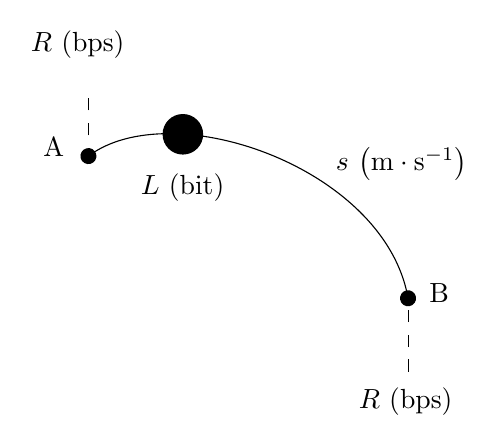
\begin{tikzpicture}[x=0.75pt,y=0.75pt,yscale=-1,xscale=1]
        %uncomment if require: \path (0,300); %set diagram left start at 0, and has height of 300
        
        %Curve Lines [id:da6142230575174562] 
        \draw    (100,118) .. controls (140,88) and (243,123.5) .. (254,186.5) ;
        \draw [shift={(254,186.5)}, rotate = 80.1] [color={rgb, 255:red, 0; green, 0; blue, 0 }  ][fill={rgb, 255:red, 0; green, 0; blue, 0 }  ][line width=0.75]      (0, 0) circle [x radius= 3.35, y radius= 3.35]   ;
        \draw [shift={(100,118)}, rotate = 323.13] [color={rgb, 255:red, 0; green, 0; blue, 0 }  ][fill={rgb, 255:red, 0; green, 0; blue, 0 }  ][line width=0.75]      (0, 0) circle [x radius= 3.35, y radius= 3.35]   ;
        %Shape: Circle [id:dp6246733531959744] 
        \draw  [fill={rgb, 255:red, 0; green, 0; blue, 0 }  ,fill opacity=1 ] (136,107.5) .. controls (136,102.25) and (140.25,98) .. (145.5,98) .. controls (150.75,98) and (155,102.25) .. (155,107.5) .. controls (155,112.75) and (150.75,117) .. (145.5,117) .. controls (140.25,117) and (136,112.75) .. (136,107.5) -- cycle ;
        %Straight Lines [id:da5479562393534617] 
        \draw  [dash pattern={on 4.5pt off 4.5pt}]  (100,120) -- (100,84.5) ;
        
        %Straight Lines [id:da2224114279600633] 
        \draw  [dash pattern={on 4.5pt off 4.5pt}]  (254,222) -- (254,186.5) ;
        
        % Text Node
        \draw (77,108) node [anchor=north west][inner sep=0.75pt]   [align=left] {A};
        % Text Node
        \draw (263,178) node [anchor=north west][inner sep=0.75pt]   [align=left] {B};
        % Text Node
        \draw (124,125.4) node [anchor=north west][inner sep=0.75pt]    {$L\mathrm{\ ( bit)}$};
        % Text Node
        \draw (71,56.4) node [anchor=north west][inner sep=0.75pt]    {$R\mathrm{\ ( bps)}$};
        % Text Node
        \draw (229,228.4) node [anchor=north west][inner sep=0.75pt]    {$R\mathrm{\ ( bps)}$};
        % Text Node
        \draw (218,112.4) node [anchor=north west][inner sep=0.75pt]    {$s\mathrm{\ \left( m\cdot s^{-1}\right)}$};
        
        
        \end{tikzpicture}
    \end{figure}
    \begin{enumerate}[label={$\left.\mathrm{\alph*}\right)$}, itemsep=0pt]
        \item 用 $m$ 和 $s$ 来表示传播时延 $d_\mathrm{prop}$.
        \begin{sol}
            根据传播时延的定义可知, 传播时延是节点间距离与传播速度的比值, 即
            $d_\mathrm{prop} = m/s$.
        \end{sol}
        \item 用 $L$ 和 $R$ 来表示该分组的传输时间 $t_\mathrm{trans}$.
        \begin{sol}
            传输时延是指数据从节点被推入通信链路中所花的时间,
            它是数据长度与链路传输速率的比值, 因此 $d_\mathrm{trans} = L/R$.
            % 由于数据传输到 B 节点后进入主机 B 也需要时间, 因此本题中所要求的时间\footnote{
            %     为了避免混淆, 原题目中的传播时间 $d_\mathrm{trans}$ 
            %     在此处记作 $t_\mathrm{trans}$, 记号 $d_\mathrm{trans}$ 
            %     仅用来表示一个分组穿过节点与链路的分界面的时间, 下同.
            % }
            % $t_\mathrm{trans} = 2d_\mathrm{trans} = 2L/R$.
        \end{sol}
        \item 忽略处理和排队时延, 得出端到端时延的表达式.
        \begin{sol}
            在该问题中, 端到端时延由传输时延和传播时延两部分组成, 而这两个部分
            在前两问中都已经计算过了, 因此
            \[ d_\mathrm{end-end} = d_\mathrm{prop} + d_\mathrm{trans}
            = \dfrac{m}{s} + \dfrac{L}{R}. \]
        \end{sol}
        \item 假定主机 A 在时刻 $t=0$ 开始传输该分组, 在时刻 $t = t_\mathrm{trans}$,
        该分组的最后一个比特在什么地方?
        \begin{sol}
            该时刻已经经历了一个传输时延, 即第一个分组已经完全传输到链路当中了.
            该分组的最后一个比特在链路中已经传播了 $d_\mathrm{trans} - d_\mathrm{trans}
            = 0$ 的时间. 在这段时间内其走过的距离为
            \[ l = s \times 0 = 0, \]
            即此时该分组的最后一个比特位于链路的 A 端点处.
        \end{sol}
        \item 假定 $d_\mathrm{prop}$ 大于 $d_\mathrm{trans}$. 
        在时刻 $t = d_\mathrm{trans}$, 该分组的第一个比特在何处?
        \begin{sol}
            根据已知条件, 该时刻该分组的第一个比特依然在链路中传播,
            由于第一个比特是直接进入链路开始传播的, 因此它已经传播了
            $d_\mathrm{trans}$ 个单位时间, 于是它所处的位置是
            $l = sd_\mathrm{trans} = sL/R$.
        \end{sol}
        \item 假定 $d_\mathrm{prop}$ 小于 $d_\mathrm{trans}$. 
        在时刻 $t = d_\mathrm{trans}$, 该分组的第一个比特在何处?
        \begin{sol}
            根据已知条件, 该时刻第一个比特已经到达 B 主机了.
        \end{sol}
    \end{enumerate}
\end{example}

\begin{example}
    考虑从主机 A 向主机 B 通过分组交换网发送语音 (VoIP). 主机 A 将模拟语音
    转换为传输中的 64kbps 数字比特流, 然后主机 A 将这些比特分为 56 字节的分组.
    A 和 B 之间有一条链路: 它的传输速率是 2Mbps, 传播时延是 10ms. 一旦 A 收集
    了一个分组, 就将它向主机 B 发送. 一旦主机 B 接收到一个完整的分组, 它将该
    分组的比特转换成模拟信号. 从比特产生 (从位于主机 A 的初始模拟信号起) 的时刻起,
    到该比特被解码 (在主机 B 上作为模拟信号的一部分), 花了多少时间?
    \begin{sol}
        我们先统一单位, 统一用比特作为单位来进行计算. 于是, 主机 A 发送的每个分组
        的大小为 $56 \times 8 = 448\si{b}$.
        这就是说, 主机 A 只需要 $448/64000$ 秒就能产生一个完整的分组, 这就是
        传输过程中的处理时延. 这就是说,
        \[ d_\mathrm{proc} 
        = \dfrac{56\si{B}}{64 \si{kbps}}
        = \dfrac{56 \times 8 \si{b}}{64 \times 10^3 \si{b \cdot s^{-1}}}
        = 7 \times 10^{-4} \si{s} =0.7 \si{ms}. \]
        \newline 接下来考虑传输时延, 事实上, 根据传输时延的定义,
        \[ d_\mathrm{trans} 
        = \dfrac{56\si{B}}{2\si{Mbps}}
        = \dfrac{56 \times 8 \si{b}}{2 \times 10^6 \si{b \cdot s^{-1}}}
        = 2.24 \times 10^{-4} \si{s} = 0.224 \si{ms}. \]
        \newline 于是最终的端到端时延为
        \[ d_\mathrm{end-end} = d_\mathrm{proc} + d_\mathrm{trans} +
        d_\mathrm{prop} = 0.7\si{ms} + 0.224 \si{ms} + 10\si{ms}
        = 10.924 \si{ms}. \]
    \end{sol}
\end{example}

\begin{example}
    假设用户共享一条 3Mbps 的链路. 又设每个用户传输时要求 150kbps, 但是
    每个用户仅有 10\% 的时间传输.
    \begin{enumerate}[label={$\left.\mathrm{\alph*}\right)$}, itemsep=0pt]
        \item 当使用电路交换时, 能够支持多少用户?
        \begin{sol}
            使用电路交换时, 每个用户都会占用一定的带宽, 因此我们可以直接用
            链路带宽和用户需求做商, 则
            \[ \mathrm{userNum} = \dfrac{3 \si{Mbps}}{150 \si{kbps}}
            = \dfrac{3 \times 10^6 \si{bps}}{150 \times 10^3 \si{bps}}
            = 20, \]
            因此在使用电路交换时, 能够支持最多 20 名用户.
        \end{sol}
        \item 当使用分组交换时, 用户正在传输的概率为?
        \begin{sol}
            由于每个用户只有 10\% 的时间传输, 所以其正在传输的概率为 0.1.
        \end{sol}
        \item 假设使用分组交换, 且有 120 名用户. 在任何给定时刻, 实际有 $n$
        个用户正在传输的概率是?
        \begin{sol}
            显然, 我们可以将这个问题视为连续进行 120 次随机事件发生概率为 0.1 
            的 Bernoulli 试验,
            正在传输数据的用户数量 $X \sim B(0.1, 120)$. 那么
            \[ P(X = n) = \mathrm{C}_{120}^n \times 0.1^n
            \times 0.9{120-n}. \]
            其中 $\mathrm{C}_m^k = \binom{m}{k}$ 为组合数, 即有限集合 $A$
            ($A$ 中含有 $m$ 个元素, 记作 $|A| = m$)
            的满足 $|S| = k$ 的子集 $S \subset A$ 的数量.
        \end{sol}
    \end{enumerate}
\end{example}

\begin{example}
    在一个电路交换网络中, 每台端系统与一台交换机直接相连, 当两台端系统要通信时, 该网络在两台
    端系统之间建立一条专用的端到端连接.
    用户在忙时以 1000kbps 的速率产生数据, 但忙时仅以 $p=0.1$ 的概率产生数据,
    假定电路交换链路的带宽为 1Gbps.
    \begin{enumerate}[label={$\left.\mathrm{\alph*}\right)$}, itemsep=0pt]
        \item 在采用电路交换技术时, 能被支持的最大用户数量 $N$ 是多少?
        \begin{sol}
            可以用链路带宽与用户需求带宽做商直接得到能够支持的最大用户数量
            \[ N = \dfrac{1\si{Gbps}}{100\si{kbps}}
            = \dfrac{1 \times 10^9 \si{bps}}{100 \times 10^3 \si{bps}}
            = 10^4. \]
        \end{sol}
        \item 在使用分组交换时, 假设有 $M$ 个用户, 多于 $N$ 个用户发送数据
        的概率为?
        \begin{sol}
            设正在发生数据的用户数量为 $X$, 显然 $X \sim B(0.1, M)$. 同时,
            由于两个用户发送数据与否是独立的, 因此
            随机事件 $\left\{ X=N+1 \right\},
            \left\{ X=N+2 \right\},
            \cdots,
            \left\{ X=M \right\}$
            是随机事件 $\left\{ X>N \right\}$ 的一个划分, 由全概率公式得
            \[ P(X>N) = \sum_{k=N+1}^{M} P(X=k)
            = \sum_{k=N+1}^{M} \mathrm{C}_M^k \times 0.1^k \times 0.9^{M-k}. \]
        \end{sol}
    \end{enumerate}
\end{example}

\begin{example}
    令 $a$ 表示在一条链路上分组的到达率, 其单位为 $\si{pkt/s}$, $\mu$ 为
    一条链路上分组的传输率, 基于 $d = d_\mathrm{queue} + d_\mathrm{trans}$,
    用 $a$ 和 $\mu$ 表示 $d$.
    \begin{sol}
        要用 $a$ 和 $\mu$ 表示 $d$, 只需用 $a$ 和 $\mu$ 表示
        $d_\mathrm{queue}$ 和 $d_\mathrm{trans}$. 我们只考虑 $1$ 个分组, 那么
        \[ d_\mathrm{queue} = \dfrac{1}{a}, \quad 
        d_\mathrm{trans} = \dfrac{1}{\mu}. \]
        于是总时延
        \[ d = \dfrac{1}{a} + \dfrac{1}{\mu}. \]
    \end{sol}
\end{example}

Little 公式是排队论中的一个著名公式, 设 $N$ 是传输队列中待传输分组的平均数量,
$a$ 为分组到达率, $d$ 为一个分组经历的平均总时延 (即排队时延加传输时延).
Little 公式表明,
\[ N = ad. \]
其实呢, Little 公式的意思就是说, 每分钟有 $a$ 个人来排队,
处理一个人平均需要 $d$ 分钟, 那么这个队伍的长度就应该是 $ad$.



\begin{example}
    考虑一台路由器缓存前面的一条出链路. 假定某队列平均包含 10 个分组, 
    平均分组排队时延是 10ms, 链路传输速率为 100pkt/s.
    不考虑丢包情况, 使用 Little 公式计算平均分组到达率.
    \begin{sol}
        由已知条件, $N = 10$, $d_\mathrm{queue} = 10\si{ms}$,
        $d_\mathrm{trans} = \dfrac{1}{100} \si{s}$, 那么
        \[ N = a d 
        = a \left( d_\mathrm{queue} + d_\mathrm{trans} \right), \]
        代入数值,
        \[ 
        \begin{aligned}
            10 \si{pkt} 
            &= a \si{pkt/s} \left(
                10\si{ms} + \dfrac{1}{100}\si{s}
            \right) 
            = a \si{pkt/s} \left(
                \dfrac{1}{100} \si{s} + \dfrac{1}{100}\si{s}
            \right) \\ 
            & = a \times 0.02 \si{s},
        \end{aligned} \]
        解得平均分组到达率 $a = 10/0.02 = 500 \si{pkt/s}$.
    \end{sol}
\end{example}

\begin{example}
    假设你希望从波士顿向洛杉矶紧急传送 $40 \times 10^{12} \si{B}$ 的数据,
    你有一条 $1\si{Gbps}$ 的专用链路可用于传输数据. 你是愿意通过这条链路传输
    数据, 还是愿意使用 FedEx 夜间快递来交付?
    \begin{sol}
        FedEx 夜间快递是指 FedEx 提供的在晚间送达包裹的服务,
        这种服务通常适用于那些需要在次日早晨或者特定时间内送达的包裹\footnote{
            这段材料由 ChatGPT 生成, ChatGPT 可能会生成错误的信息, 请谨慎参考.
        }. 
        我们不妨假设 FedEx 可以在 72 小时内将包裹送达洛杉矶.
        那么使用专用链路的传输时间 
        \[ 
        \begin{aligned}
            t &= \dfrac{40 \times 10^{12} \si{B}}{1 \si{Gbps}}
            = \dfrac{8 \times 40 \times 10^{12} \si{b}}{10^9 \si{bps}} \\ 
            &= 320,000 \si{s} = \dfrac{320,000 \si{s}}{3600 \si{s/h}} 
            \approx 89 \si{h} > 72 \si{h}.
        \end{aligned} \]
        于是我选择 FedEx 夜间快递.
    \end{sol}
\end{example}

\begin{example}
    在包括因特网的现代分组交换网络中, 源端系统将长应用层报文分段为较小的分组并向
    网络发送, 接收方将这些分组重新装配为原始报文, 这个过程称为报文分段.
    考虑一个长度为 $8 \times 10^6 \si{bit}$ 的报文, 经过两个分组交换机
    到达目的端系统, 每段链路的传输速率是 $2 \si{Mbps}$. 忽略传播、排队和处理
    时延.
    \begin{enumerate}[label={$\left.\mathrm{\alph*}\right)$}, itemsep=0pt]
        \item 考虑从源端系统到目的端系统发送该报文且没有报文分段, 从源端系统到
        第一台分组交换机需要多长时间? (每台分组交换机均适用存储转发分组交换)
        从源端系统移动该报文到目的端系统需要多长时间?
        \begin{sol}
            没有报文分段时, 从源端系统到第一台分组交换机需要的时间为
            \[ t_1 = \frac{8 \times 10^6 \si{bit}}{2 \si{Mbps}} = 4\si{s}, \]
        该文件最终到达目的端系统的时间为
        \[ t = 3t_1 = 12 \si{s}. \]
        \end{sol}
        \item 假设报文被分段为 800 个分组, 每个分组长度为 $10,000\si{bit}$.
        从源端系统移动第一个分组到第一个分组交换机需要多长时间? 从第一台交换机发送
        第一个分组到第二台交换机, 从源端系统发送第二个分组到第一台交换机各需要多长时间?
        什么时候第二个分组能被第一台交换机全部收到?
        \begin{sol}
            有报文分段时, 从源端系统移动第一个分组到第一台分组交换机需要的时间为
            \[ t_1' = \frac{10,000 \si{bit}}{2 \si{Mbps}} = 5\si{ms} \]
            由于每个分组的传输速率相同, 且不考虑出了传输时延以外的各种时延,
            因此从第一台交换机到第二个交换机需要 $t_1'$ 时间,
            第二个分组源端系统到第一台交换机需要 $t_1'$ 时间.
            于是在整个过程经历 $2t_1'$, 即 $10\si{ms}$ 后, 第二个分组被
            第一台交换机全部收到.
        \end{sol}
        \item 使用报文分段时, 该文件从源端系统到目的端系统需要多长时间?
        \begin{sol}
            每个分组需要 $3t_1'$ 的时间才能完全送到目的端系统, 但是由于在整个过程中
            三条链路都在不停地传输数据, 因此事实上传输 800 个分组只需要 $(800+2)t_1$
            的时间, 这是因为我们需要 $2t_1$ 的时间才能让三条链路全部工作起来.
            所以他需要的时间为
            \[ t' = (800+2) \times 5\si{ms} = 4010 \si{ms} < 4\si{s}, \]
            发现使用报文分段时, 传输速率能够大幅减小时延.
        \end{sol}
        \item 除了减小时延以外, 使用报文分段还有什么原因?
        \begin{sol}
            除了减小时延以外, 使用报文分段还能够提高链路的使用率. 事实上,
            在不使用报文分段的时候, 传输的第二阶段 (即从交换机 1 到交换机 2)
            是源端系统到交换机 1 的链路和交换机 2 到目的端系统的链路是空闲的.
            在传输的第一阶段和第三阶段同理, 而当网络中接入的用户数量增加,
            链路的利用率将会变得至关重要, 因此采用报文分段的方式.
        \end{sol}
        \item 讨论报文分段的缺点.
        \begin{itemize}[itemsep=0pt]
            \item 由于报文分段把一段报文分解为若干分组, 因此在拆分报文和重组报文
            的过程中会产生一定的时间开销;
            \item 由于分组当中包含一些头部信息, 所以报文分段会产生额外的头部信息, 
            增加了传输数据量; 
            \item 分组在遇到丢包
            的时候需要重传 (虽然重传一个分组总比重传一整个文件更容易, 但是若干个
            分组中有一个分组丢包的概率是要远远大于 1 整个文件丢包的概率的);
            \item 报文分段可能会降低实时性.
        \end{itemize}
    \end{enumerate}
\end{example}

\newpage
\thispagestyle{empty}

\chapter{应用层}

本章的主要任务是:
\begin{tasks}
    \task 定义关键的应用层概念 (网络服务、客户、服务器、进程、运输层接口);
    \task 详细考察几种网络应用程序 (Web、电子邮件、DNS、对等文件分发)
\end{tasks}

\section{网络应用原理}

% \subsection{将应用程序限制在端系统的思想}

研发网络应用程序的核心是写出能够运行在不同端系统和通过网络彼此通信的程序,
这个程序应该能在多个端系统上运行, 但并不需要在网络核心设备 (路由器、链路层交换机)
上运行. 于是, 网络应用程序被限制在了网络边缘, 而网络核心设备并不在应用层起作用.

\subsection{网络应用体系结构}

\textbf{应用体系结构} (application architecture) 是由应用程序研发者设计的,
规定了如何在各种端系统上组织该应用程序的体系结构. 本小节介绍两种主流的网络应用
体系结构: \textbf{客户—服务器体系结构} (client-server architecture, C-S) 
和\textbf{对等体系结构} (P2P architecture, P2P).

在这里要强调的是, 网络应用程序的体系结构不等同于网络的体系结构, 因特网的协议栈自
顶向下分别是应用层、传输层、网络层、链路层和物理层, 它为应用程序提供了特定的服务的
集合. 请诸位读者注意这两个概念的区别.

\subsubsection{客户—服务器体系结构 (C-S 结构)}



在 C-S 结构当中, 有一个总是打开的端系统, 我们称之为\textbf{服务器} (server),
它服务于来自许多称之为\textbf{客户} (client) 的端系统的\textbf{请求} (request).
C-S 结构的主要特点为:
\begin{enumerate}[itemsep=0pt, label={$\left.\mathrm{\alph*}\right)$}]
    \item 客户之间不相互通信;
    \item 服务器具有固定的、公开的地址, 我们将其称之为 IP 地址.
\end{enumerate}
由于服务器的地址固定、公开, 且服务器总是打开的, 所以客户才能够向服务器的 IP 地址发送分组
来取得联系.

\begin{example}
    Web 应用程序是典型的具有客户—服务器体系结构的网络应用程序. Web 服务器服务于
    来自运行在客户的主机上的浏览器的请求, 当 Web 服务器接收到请求时, 它向客户发送
    所请求的对象, 这个过程称为\textbf{响应}. 在 Web 应用中, 两个客户的浏览器并不
    直接通信, 这也符合 C-S 体系结构的特征.
\end{example}
\begin{example}
    我们很快就会看到,
    FTP、Telnet、电子邮件也是具有 C-S 体系结构的典型的网络应用程序.
\end{example}

\begin{figure}[H]
    \centering


\tikzset{every picture/.style={line width=0.75pt}} %set default line width to 0.75pt        

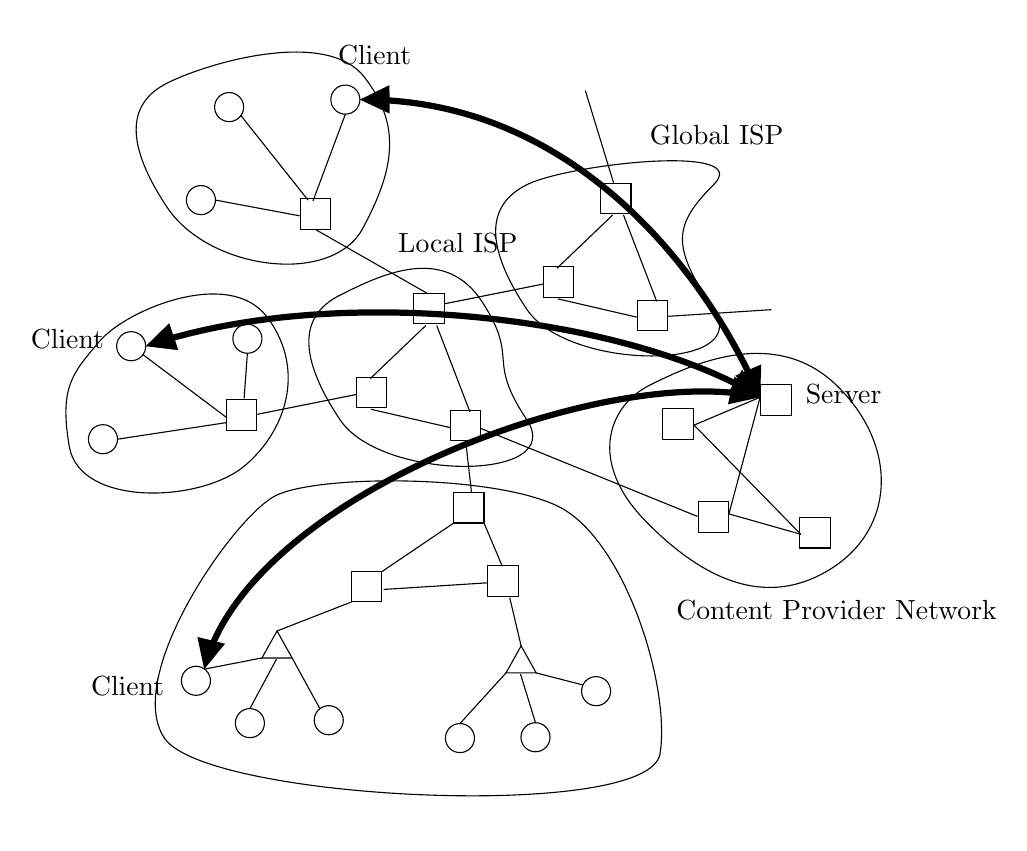
\begin{tikzpicture}[x=0.75pt,y=0.75pt,yscale=-1,xscale=1]
%uncomment if require: \path (0,444); %set diagram left start at 0, and has height of 444

%Shape: Circle [id:dp433612958331524] 
\draw   (123.8,69) .. controls (123.8,65.13) and (126.93,62) .. (130.8,62) .. controls (134.67,62) and (137.8,65.13) .. (137.8,69) .. controls (137.8,72.87) and (134.67,76) .. (130.8,76) .. controls (126.93,76) and (123.8,72.87) .. (123.8,69) -- cycle ;
%Shape: Circle [id:dp9525464000680568] 
\draw   (110.2,113.8) .. controls (110.2,109.93) and (113.33,106.8) .. (117.2,106.8) .. controls (121.07,106.8) and (124.2,109.93) .. (124.2,113.8) .. controls (124.2,117.67) and (121.07,120.8) .. (117.2,120.8) .. controls (113.33,120.8) and (110.2,117.67) .. (110.2,113.8) -- cycle ;
%Shape: Circle [id:dp907243927480952] 
\draw   (179.8,65.4) .. controls (179.8,61.53) and (182.93,58.4) .. (186.8,58.4) .. controls (190.67,58.4) and (193.8,61.53) .. (193.8,65.4) .. controls (193.8,69.27) and (190.67,72.4) .. (186.8,72.4) .. controls (182.93,72.4) and (179.8,69.27) .. (179.8,65.4) -- cycle ;
%Shape: Square [id:dp3698725273485206] 
\draw   (165,113.2) -- (179.6,113.2) -- (179.6,127.8) -- (165,127.8) -- cycle ;
%Straight Lines [id:da0969726034637598] 
\draw    (124.2,113.8) -- (164.8,121.4) ;
%Straight Lines [id:da08552766598631123] 
\draw    (136.4,73) -- (168.8,113.8) ;
%Straight Lines [id:da3217379254695535] 
\draw    (186.8,72.4) -- (171.2,114.2) ;
%Shape: Square [id:dp4178698813728665] 
\draw   (219.8,158.8) -- (234.4,158.8) -- (234.4,173.4) -- (219.8,173.4) -- cycle ;
%Shape: Square [id:dp6333689045183972] 
\draw   (192.2,199.2) -- (206.8,199.2) -- (206.8,213.8) -- (192.2,213.8) -- cycle ;
%Shape: Square [id:dp021929665571026824] 
\draw   (237.4,215.2) -- (252,215.2) -- (252,229.8) -- (237.4,229.8) -- cycle ;
%Shape: Polygon Curved [id:ds8620606985361757] 
\draw   (101,57.4) .. controls (121,47.4) and (177.8,31) .. (196,54.6) .. controls (214.2,78.2) and (210.2,99.4) .. (195.2,127.4) .. controls (180.2,155.4) and (121,147.4) .. (101,117.4) .. controls (81,87.4) and (81,67.4) .. (101,57.4) -- cycle ;
%Shape: Polygon Curved [id:ds05829423855221605] 
\draw   (184.2,159.6) .. controls (204.2,149.6) and (234.6,134.8) .. (252.8,163) .. controls (271,191.2) and (254.2,189.6) .. (274.2,219.6) .. controls (294.2,249.6) and (204.2,249.6) .. (184.2,219.6) .. controls (164.2,189.6) and (164.2,169.6) .. (184.2,159.6) -- cycle ;
%Straight Lines [id:da14534134927089626] 
\draw    (225.6,174.2) -- (198.8,199.8) ;
%Straight Lines [id:da5712582233280207] 
\draw    (230.8,174.2) -- (246.8,215.8) ;
%Straight Lines [id:da38655135659204964] 
\draw    (199.2,214.6) -- (237.2,223.4) ;
%Shape: Circle [id:dp261308081277286] 
\draw   (76.6,184.2) .. controls (76.6,180.33) and (79.73,177.2) .. (83.6,177.2) .. controls (87.47,177.2) and (90.6,180.33) .. (90.6,184.2) .. controls (90.6,188.07) and (87.47,191.2) .. (83.6,191.2) .. controls (79.73,191.2) and (76.6,188.07) .. (76.6,184.2) -- cycle ;
%Shape: Circle [id:dp11198982335928176] 
\draw   (63,229) .. controls (63,225.13) and (66.13,222) .. (70,222) .. controls (73.87,222) and (77,225.13) .. (77,229) .. controls (77,232.87) and (73.87,236) .. (70,236) .. controls (66.13,236) and (63,232.87) .. (63,229) -- cycle ;
%Shape: Circle [id:dp3855756046665245] 
\draw   (132.6,180.6) .. controls (132.6,176.73) and (135.73,173.6) .. (139.6,173.6) .. controls (143.47,173.6) and (146.6,176.73) .. (146.6,180.6) .. controls (146.6,184.47) and (143.47,187.6) .. (139.6,187.6) .. controls (135.73,187.6) and (132.6,184.47) .. (132.6,180.6) -- cycle ;
%Shape: Square [id:dp5640143990408383] 
\draw   (129.4,210) -- (144,210) -- (144,224.6) -- (129.4,224.6) -- cycle ;
%Straight Lines [id:da4523810651518446] 
\draw    (77,229) -- (129.6,221) ;
%Straight Lines [id:da2191344100007564] 
\draw    (89.2,188.2) -- (129.6,218.6) ;
%Straight Lines [id:da6507023685394837] 
\draw    (139.6,187.6) -- (138,209.4) ;
%Shape: Polygon Curved [id:ds07952252277659255] 
\draw   (68.4,181.8) .. controls (81.2,166.6) and (130.6,146.2) .. (148.8,169.8) .. controls (167,193.4) and (160,223) .. (138.8,241.4) .. controls (117.6,259.8) and (58.8,261.8) .. (53.8,232.6) .. controls (48.8,203.4) and (55.6,197) .. (68.4,181.8) -- cycle ;
%Straight Lines [id:da021050973019674957] 
\draw    (172.8,128.2) -- (226,158.6) ;
%Straight Lines [id:da7073775090814787] 
\draw    (144.4,217) -- (192.4,207.4) ;
%Shape: Square [id:dp18469887748978797] 
\draw   (239,254.8) -- (253.6,254.8) -- (253.6,269.4) -- (239,269.4) -- cycle ;
%Shape: Square [id:dp3224913332890308] 
\draw   (189.8,292.8) -- (204.4,292.8) -- (204.4,307.4) -- (189.8,307.4) -- cycle ;
%Shape: Square [id:dp6259173434159957] 
\draw   (255.4,290) -- (270,290) -- (270,304.6) -- (255.4,304.6) -- cycle ;
%Straight Lines [id:da13535192196926238] 
\draw    (204.4,292.8) -- (239,269.4) ;
%Straight Lines [id:da743800514125592] 
\draw    (262.4,290.2) -- (253.6,269.4) ;
%Straight Lines [id:da7006325233979058] 
\draw    (255.2,298.2) -- (205.2,301.4) ;
%Straight Lines [id:da151354382232873] 
\draw    (244.8,230.2) -- (247.6,255) ;
%Flowchart: Extract [id:dp07545426293354496] 
\draw   (153.87,321.4) -- (161.14,334.4) -- (146.6,334.4) -- cycle ;
%Shape: Circle [id:dp8135801241855177] 
\draw   (107.8,345.4) .. controls (107.8,341.53) and (110.93,338.4) .. (114.8,338.4) .. controls (118.67,338.4) and (121.8,341.53) .. (121.8,345.4) .. controls (121.8,349.27) and (118.67,352.4) .. (114.8,352.4) .. controls (110.93,352.4) and (107.8,349.27) .. (107.8,345.4) -- cycle ;
%Shape: Circle [id:dp4005105760383596] 
\draw   (133.8,365.8) .. controls (133.8,361.93) and (136.93,358.8) .. (140.8,358.8) .. controls (144.67,358.8) and (147.8,361.93) .. (147.8,365.8) .. controls (147.8,369.67) and (144.67,372.8) .. (140.8,372.8) .. controls (136.93,372.8) and (133.8,369.67) .. (133.8,365.8) -- cycle ;
%Shape: Circle [id:dp8438243992018043] 
\draw   (171.8,364.4) .. controls (171.8,360.53) and (174.93,357.4) .. (178.8,357.4) .. controls (182.67,357.4) and (185.8,360.53) .. (185.8,364.4) .. controls (185.8,368.27) and (182.67,371.4) .. (178.8,371.4) .. controls (174.93,371.4) and (171.8,368.27) .. (171.8,364.4) -- cycle ;
%Straight Lines [id:da35690531414982074] 
\draw    (118.8,339.8) -- (146.6,334.4) ;
%Straight Lines [id:da8966008111874162] 
\draw    (140.8,358.8) -- (153.6,335) ;
%Straight Lines [id:da24938101448418315] 
\draw    (174.4,358.6) -- (161.14,334.4) ;
%Straight Lines [id:da11533719279073273] 
\draw    (189.8,307.4) -- (153.87,321.4) ;
%Flowchart: Extract [id:dp31062992908616816] 
\draw   (271.47,328.6) -- (278.74,341.6) -- (264.2,341.6) -- cycle ;
%Shape: Circle [id:dp8225120151872738] 
\draw   (235,373) .. controls (235,369.13) and (238.13,366) .. (242,366) .. controls (245.87,366) and (249,369.13) .. (249,373) .. controls (249,376.87) and (245.87,380) .. (242,380) .. controls (238.13,380) and (235,376.87) .. (235,373) -- cycle ;
%Shape: Circle [id:dp8396413941712775] 
\draw   (271.4,372.6) .. controls (271.4,368.73) and (274.53,365.6) .. (278.4,365.6) .. controls (282.27,365.6) and (285.4,368.73) .. (285.4,372.6) .. controls (285.4,376.47) and (282.27,379.6) .. (278.4,379.6) .. controls (274.53,379.6) and (271.4,376.47) .. (271.4,372.6) -- cycle ;
%Shape: Circle [id:dp6585240742001846] 
\draw   (300.6,350.4) .. controls (300.6,346.53) and (303.73,343.4) .. (307.6,343.4) .. controls (311.47,343.4) and (314.6,346.53) .. (314.6,350.4) .. controls (314.6,354.27) and (311.47,357.4) .. (307.6,357.4) .. controls (303.73,357.4) and (300.6,354.27) .. (300.6,350.4) -- cycle ;
%Straight Lines [id:da2650143855067648] 
\draw    (242,366) -- (264.2,341.6) ;
%Straight Lines [id:da30082251672054805] 
\draw    (278.4,365.6) -- (271.2,342.2) ;
%Straight Lines [id:da1768508112270082] 
\draw    (301.2,347.4) -- (278.74,341.6) ;
%Straight Lines [id:da6321152470144745] 
\draw    (266,305.4) -- (271.47,328.6) ;
%Shape: Polygon Curved [id:ds1617692645912968] 
\draw   (153.2,256.2) .. controls (173.2,246.2) and (256,245.8) .. (288.6,261) .. controls (321.2,276.2) and (343.6,347.8) .. (338.4,380.6) .. controls (333.2,413.4) and (119.6,403) .. (99.6,373) .. controls (79.6,343) and (133.2,266.2) .. (153.2,256.2) -- cycle ;
%Shape: Square [id:dp08663806294800447] 
\draw   (309.8,105.6) -- (324.4,105.6) -- (324.4,120.2) -- (309.8,120.2) -- cycle ;
%Shape: Square [id:dp9147693818266068] 
\draw   (282.2,146) -- (296.8,146) -- (296.8,160.6) -- (282.2,160.6) -- cycle ;
%Shape: Square [id:dp15237094785941618] 
\draw   (327.4,162) -- (342,162) -- (342,176.6) -- (327.4,176.6) -- cycle ;
%Shape: Polygon Curved [id:ds5863532904886407] 
\draw   (274.2,106.4) .. controls (294.2,96.4) and (384.2,86.4) .. (364.2,106.4) .. controls (344.2,126.4) and (344.2,136.4) .. (364.2,166.4) .. controls (384.2,196.4) and (294.2,196.4) .. (274.2,166.4) .. controls (254.2,136.4) and (254.2,116.4) .. (274.2,106.4) -- cycle ;
%Straight Lines [id:da5129218701921046] 
\draw    (315.6,121) -- (288.8,146.6) ;
%Straight Lines [id:da8333338125419416] 
\draw    (320.8,121) -- (336.8,162.6) ;
%Straight Lines [id:da8143993028354376] 
\draw    (289.2,161.4) -- (327.2,170.2) ;
%Straight Lines [id:da5923387128997158] 
\draw    (302.4,61) -- (316,105.4) ;
%Straight Lines [id:da33598274330973965] 
\draw    (234.4,163.8) -- (282.4,154.2) ;
%Shape: Square [id:dp4267098814927107] 
\draw   (339.8,214.4) -- (354.4,214.4) -- (354.4,229) -- (339.8,229) -- cycle ;
%Shape: Square [id:dp9240413294855849] 
\draw   (357,259.2) -- (371.6,259.2) -- (371.6,273.8) -- (357,273.8) -- cycle ;
%Straight Lines [id:da32322730905764274] 
\draw    (354.8,222.2) -- (386.6,208.8) ;
%Straight Lines [id:da8910209006572074] 
\draw    (354.8,222.2) -- (406.2,274.8) ;
%Straight Lines [id:da22522589201955268] 
\draw    (371.6,265) -- (386.6,208.8) ;
%Straight Lines [id:da5365393724473647] 
\draw    (371.6,265) -- (406.2,274.8) ;
%Shape: Square [id:dp4662017797946353] 
\draw   (387,202.8) -- (401.6,202.8) -- (401.6,217.4) -- (387,217.4) -- cycle ;
%Shape: Square [id:dp51343497776989] 
\draw   (405.8,266.8) -- (420.4,266.8) -- (420.4,281.4) -- (405.8,281.4) -- cycle ;
%Straight Lines [id:da030520013480400232] 
\draw    (252,223.8) -- (356.4,266.2) ;
%Shape: Polygon Curved [id:ds15357211830032558] 
\draw   (333.4,203) .. controls (353.4,193) and (393.6,174.2) .. (423.4,203) .. controls (453.2,231.8) and (452,271.8) .. (420.8,291.4) .. controls (389.6,311) and (358.8,296.6) .. (331.2,268.2) .. controls (303.6,239.8) and (313.4,213) .. (333.4,203) -- cycle ;
%Straight Lines [id:da1476417292163149] 
\draw    (342.4,169.8) -- (392,166.6) ;
%Curve Lines [id:da15121399208877162] 
\draw [line width=2.25]    (199.83,65.44) .. controls (295.59,67.69) and (357.06,143.64) .. (384.94,205.06) ;
\draw [shift={(386.6,208.8)}, rotate = 246.44] [fill={rgb, 255:red, 0; green, 0; blue, 0 }  ][line width=0.08]  [draw opacity=0] (14.29,-6.86) -- (0,0) -- (14.29,6.86) -- cycle    ;
\draw [shift={(193.8,65.4)}, rotate = 359.49] [fill={rgb, 255:red, 0; green, 0; blue, 0 }  ][line width=0.08]  [draw opacity=0] (14.29,-6.86) -- (0,0) -- (14.29,6.86) -- cycle    ;
%Curve Lines [id:da600088945952852] 
\draw [line width=2.25]    (96.26,182.36) .. controls (187.7,153.81) and (319.84,170.56) .. (382.83,206.57) ;
\draw [shift={(386.6,208.8)}, rotate = 211.46] [fill={rgb, 255:red, 0; green, 0; blue, 0 }  ][line width=0.08]  [draw opacity=0] (14.29,-6.86) -- (0,0) -- (14.29,6.86) -- cycle    ;
\draw [shift={(90.6,184.2)}, rotate = 341.25] [fill={rgb, 255:red, 0; green, 0; blue, 0 }  ][line width=0.08]  [draw opacity=0] (14.29,-6.86) -- (0,0) -- (14.29,6.86) -- cycle    ;
%Curve Lines [id:da2349834302643008] 
\draw [line width=2.25]    (120.19,334.82) .. controls (145.41,255.55) and (307.79,194.34) .. (382.16,207.88) ;
\draw [shift={(386.6,208.8)}, rotate = 193.23] [fill={rgb, 255:red, 0; green, 0; blue, 0 }  ][line width=0.08]  [draw opacity=0] (14.29,-6.86) -- (0,0) -- (14.29,6.86) -- cycle    ;
\draw [shift={(118.8,339.8)}, rotate = 283.63] [fill={rgb, 255:red, 0; green, 0; blue, 0 }  ][line width=0.08]  [draw opacity=0] (14.29,-6.86) -- (0,0) -- (14.29,6.86) -- cycle    ;

% Text Node
\draw (211,128.6) node [anchor=north west][inner sep=0.75pt]   [align=left] {Local ISP};
% Text Node
\draw (332.2,76.6) node [anchor=north west][inner sep=0.75pt]   [align=left] {Global ISP};
% Text Node
\draw (407.4,201.6) node [anchor=north west][inner sep=0.75pt]   [align=left] {Server};
% Text Node
\draw (345,305.2) node [anchor=north west][inner sep=0.75pt]   [align=left] {Content Provider Network};
% Text Node
\draw (34,175) node [anchor=north west][inner sep=0.75pt]   [align=left] {Client};
% Text Node
\draw (182,38) node [anchor=north west][inner sep=0.75pt]   [align=left] {Client};
% Text Node
\draw (63,342) node [anchor=north west][inner sep=0.75pt]   [align=left] {Client};


\end{tikzpicture}
\caption{客户—服务器体系结构 (Client-Server Architecture)}
\end{figure}


\subsubsection{对等体系结构 (P2P 结构)}

P2P 体系结构中的用户需要通信时, 不需要通过专门的服务器,
而是可以直接与对方的主机通信, 相互通信的双方被称为\textbf{对等方}. 
这种结构对专用服务器具有最小的依赖, 有时甚至没有依赖, 它的主要特征为:
\begin{enumerate}[itemsep=0pt, label={$\left.\mathrm{\alph*}\right)$}]
    \item \textbf{自扩展性} (self-scalability): 每个对等方的加入在占用网络资源
    的同时也在增加系统的服务能力;
    \item \textbf{有成本效率}: P2P 体系结构的网络应用程序不需要庞大的服务器基础设施
    和服务器带宽.
    \item \textbf{风险与挑战}: P2P 应用程序的非集中式结构在降低服务器成本的同时也
    带来了安全性、性能和可靠性等多方面的挑战. 
\end{enumerate}

\begin{example}
    服务程序在 Windows 环境下工作, 并且运行该服务器的计算机也作为客户访问其他计算机
    提供的服务, 那么, 这种网络应用模型属于 \underline{\qquad \qquad \qquad}.
    \begin{tasks}[label={\Alph*.}](2)
        \task 主从式 (master-slave architecture)
        \task 对等式
        \task 客户/服务器模型
        \task 集中式
    \end{tasks}
    \begin{cmt}
        “运行该服务器的计算机也作为客户访问其他计算机提供的服务” 说明在这个网络应用
        模型中并没有固定的客户与服务器的划分, 属于 P2P 模式, 因此本题选择 B 选项.
        P2P 模型中各用户
        的计算机共享资源, 从而提供比单个用户所能提供的多得多的资源, 任意一对计算机
        被称为对等方.
    \end{cmt}
\end{example}

\begin{figure}[H]
    \centering


\tikzset{every picture/.style={line width=0.75pt}} %set default line width to 0.75pt        

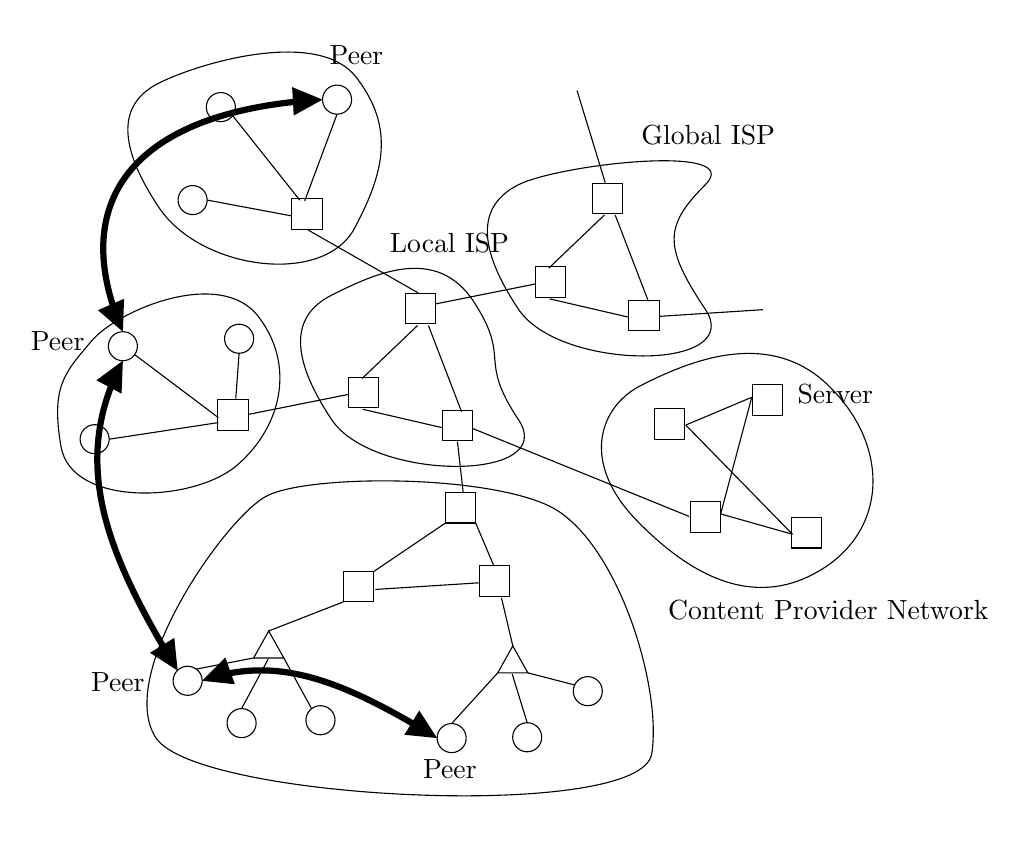
\begin{tikzpicture}[x=0.75pt,y=0.75pt,yscale=-1,xscale=1]
%uncomment if require: \path (0,435); %set diagram left start at 0, and has height of 435

%Shape: Circle [id:dp1668017344196715] 
\draw   (143.8,69) .. controls (143.8,65.13) and (146.93,62) .. (150.8,62) .. controls (154.67,62) and (157.8,65.13) .. (157.8,69) .. controls (157.8,72.87) and (154.67,76) .. (150.8,76) .. controls (146.93,76) and (143.8,72.87) .. (143.8,69) -- cycle ;
%Shape: Circle [id:dp7126289694631196] 
\draw   (130.2,113.8) .. controls (130.2,109.93) and (133.33,106.8) .. (137.2,106.8) .. controls (141.07,106.8) and (144.2,109.93) .. (144.2,113.8) .. controls (144.2,117.67) and (141.07,120.8) .. (137.2,120.8) .. controls (133.33,120.8) and (130.2,117.67) .. (130.2,113.8) -- cycle ;
%Shape: Circle [id:dp40539025391490224] 
\draw   (199.8,65.4) .. controls (199.8,61.53) and (202.93,58.4) .. (206.8,58.4) .. controls (210.67,58.4) and (213.8,61.53) .. (213.8,65.4) .. controls (213.8,69.27) and (210.67,72.4) .. (206.8,72.4) .. controls (202.93,72.4) and (199.8,69.27) .. (199.8,65.4) -- cycle ;
%Shape: Square [id:dp9799629616610039] 
\draw   (185,113.2) -- (199.6,113.2) -- (199.6,127.8) -- (185,127.8) -- cycle ;
%Straight Lines [id:da6450684922145293] 
\draw    (144.2,113.8) -- (184.8,121.4) ;
%Straight Lines [id:da5985438910431701] 
\draw    (156.4,73) -- (188.8,113.8) ;
%Straight Lines [id:da5592248873691504] 
\draw    (206.8,72.4) -- (191.2,114.2) ;
%Shape: Square [id:dp075817221394062] 
\draw   (239.8,158.8) -- (254.4,158.8) -- (254.4,173.4) -- (239.8,173.4) -- cycle ;
%Shape: Square [id:dp09626370857384847] 
\draw   (212.2,199.2) -- (226.8,199.2) -- (226.8,213.8) -- (212.2,213.8) -- cycle ;
%Shape: Square [id:dp9705969563574484] 
\draw   (257.4,215.2) -- (272,215.2) -- (272,229.8) -- (257.4,229.8) -- cycle ;
%Shape: Polygon Curved [id:ds39241928167728557] 
\draw   (121,57.4) .. controls (141,47.4) and (197.8,31) .. (216,54.6) .. controls (234.2,78.2) and (230.2,99.4) .. (215.2,127.4) .. controls (200.2,155.4) and (141,147.4) .. (121,117.4) .. controls (101,87.4) and (101,67.4) .. (121,57.4) -- cycle ;
%Shape: Polygon Curved [id:ds027187166464488266] 
\draw   (204.2,159.6) .. controls (224.2,149.6) and (254.6,134.8) .. (272.8,163) .. controls (291,191.2) and (274.2,189.6) .. (294.2,219.6) .. controls (314.2,249.6) and (224.2,249.6) .. (204.2,219.6) .. controls (184.2,189.6) and (184.2,169.6) .. (204.2,159.6) -- cycle ;
%Straight Lines [id:da10075922141073468] 
\draw    (245.6,174.2) -- (218.8,199.8) ;
%Straight Lines [id:da5871090823680505] 
\draw    (250.8,174.2) -- (266.8,215.8) ;
%Straight Lines [id:da845359291650888] 
\draw    (219.2,214.6) -- (257.2,223.4) ;
%Shape: Circle [id:dp892505781307393] 
\draw   (96.6,184.2) .. controls (96.6,180.33) and (99.73,177.2) .. (103.6,177.2) .. controls (107.47,177.2) and (110.6,180.33) .. (110.6,184.2) .. controls (110.6,188.07) and (107.47,191.2) .. (103.6,191.2) .. controls (99.73,191.2) and (96.6,188.07) .. (96.6,184.2) -- cycle ;
%Shape: Circle [id:dp3273509224935396] 
\draw   (83,229) .. controls (83,225.13) and (86.13,222) .. (90,222) .. controls (93.87,222) and (97,225.13) .. (97,229) .. controls (97,232.87) and (93.87,236) .. (90,236) .. controls (86.13,236) and (83,232.87) .. (83,229) -- cycle ;
%Shape: Circle [id:dp20627917841387589] 
\draw   (152.6,180.6) .. controls (152.6,176.73) and (155.73,173.6) .. (159.6,173.6) .. controls (163.47,173.6) and (166.6,176.73) .. (166.6,180.6) .. controls (166.6,184.47) and (163.47,187.6) .. (159.6,187.6) .. controls (155.73,187.6) and (152.6,184.47) .. (152.6,180.6) -- cycle ;
%Shape: Square [id:dp5704557413463762] 
\draw   (149.4,210) -- (164,210) -- (164,224.6) -- (149.4,224.6) -- cycle ;
%Straight Lines [id:da052928027657868415] 
\draw    (97,229) -- (149.6,221) ;
%Straight Lines [id:da018405735633047482] 
\draw    (109.2,188.2) -- (149.6,218.6) ;
%Straight Lines [id:da4852257715966948] 
\draw    (159.6,187.6) -- (158,209.4) ;
%Shape: Polygon Curved [id:ds9650415019270713] 
\draw   (88.4,181.8) .. controls (101.2,166.6) and (150.6,146.2) .. (168.8,169.8) .. controls (187,193.4) and (180,223) .. (158.8,241.4) .. controls (137.6,259.8) and (78.8,261.8) .. (73.8,232.6) .. controls (68.8,203.4) and (75.6,197) .. (88.4,181.8) -- cycle ;
%Straight Lines [id:da6949681619999016] 
\draw    (192.8,128.2) -- (246,158.6) ;
%Straight Lines [id:da5942869743526222] 
\draw    (164.4,217) -- (212.4,207.4) ;
%Shape: Square [id:dp3529302250051878] 
\draw   (259,254.8) -- (273.6,254.8) -- (273.6,269.4) -- (259,269.4) -- cycle ;
%Shape: Square [id:dp47192615376461244] 
\draw   (209.8,292.8) -- (224.4,292.8) -- (224.4,307.4) -- (209.8,307.4) -- cycle ;
%Shape: Square [id:dp42608263289747217] 
\draw   (275.4,290) -- (290,290) -- (290,304.6) -- (275.4,304.6) -- cycle ;
%Straight Lines [id:da22657141296703276] 
\draw    (224.4,292.8) -- (259,269.4) ;
%Straight Lines [id:da6423848705990195] 
\draw    (282.4,290.2) -- (273.6,269.4) ;
%Straight Lines [id:da8592821771623831] 
\draw    (275.2,298.2) -- (225.2,301.4) ;
%Straight Lines [id:da6062741219896285] 
\draw    (264.8,230.2) -- (267.6,255) ;
%Flowchart: Extract [id:dp6857773505274815] 
\draw   (173.87,321.4) -- (181.14,334.4) -- (166.6,334.4) -- cycle ;
%Shape: Circle [id:dp7538537840041853] 
\draw   (127.8,345.4) .. controls (127.8,341.53) and (130.93,338.4) .. (134.8,338.4) .. controls (138.67,338.4) and (141.8,341.53) .. (141.8,345.4) .. controls (141.8,349.27) and (138.67,352.4) .. (134.8,352.4) .. controls (130.93,352.4) and (127.8,349.27) .. (127.8,345.4) -- cycle ;
%Shape: Circle [id:dp19369727851759122] 
\draw   (153.8,365.8) .. controls (153.8,361.93) and (156.93,358.8) .. (160.8,358.8) .. controls (164.67,358.8) and (167.8,361.93) .. (167.8,365.8) .. controls (167.8,369.67) and (164.67,372.8) .. (160.8,372.8) .. controls (156.93,372.8) and (153.8,369.67) .. (153.8,365.8) -- cycle ;
%Shape: Circle [id:dp6738782230424437] 
\draw   (191.8,364.4) .. controls (191.8,360.53) and (194.93,357.4) .. (198.8,357.4) .. controls (202.67,357.4) and (205.8,360.53) .. (205.8,364.4) .. controls (205.8,368.27) and (202.67,371.4) .. (198.8,371.4) .. controls (194.93,371.4) and (191.8,368.27) .. (191.8,364.4) -- cycle ;
%Straight Lines [id:da6275389607075987] 
\draw    (138.8,339.8) -- (166.6,334.4) ;
%Straight Lines [id:da4578783518723738] 
\draw    (160.8,358.8) -- (173.6,335) ;
%Straight Lines [id:da549513383532275] 
\draw    (194.4,358.6) -- (181.14,334.4) ;
%Straight Lines [id:da08644988384767882] 
\draw    (209.8,307.4) -- (173.87,321.4) ;
%Flowchart: Extract [id:dp3932715169852613] 
\draw   (291.47,328.6) -- (298.74,341.6) -- (284.2,341.6) -- cycle ;
%Shape: Circle [id:dp5865400585855488] 
\draw   (255,373) .. controls (255,369.13) and (258.13,366) .. (262,366) .. controls (265.87,366) and (269,369.13) .. (269,373) .. controls (269,376.87) and (265.87,380) .. (262,380) .. controls (258.13,380) and (255,376.87) .. (255,373) -- cycle ;
%Shape: Circle [id:dp37175808810286814] 
\draw   (291.4,372.6) .. controls (291.4,368.73) and (294.53,365.6) .. (298.4,365.6) .. controls (302.27,365.6) and (305.4,368.73) .. (305.4,372.6) .. controls (305.4,376.47) and (302.27,379.6) .. (298.4,379.6) .. controls (294.53,379.6) and (291.4,376.47) .. (291.4,372.6) -- cycle ;
%Shape: Circle [id:dp4099594038765574] 
\draw   (320.6,350.4) .. controls (320.6,346.53) and (323.73,343.4) .. (327.6,343.4) .. controls (331.47,343.4) and (334.6,346.53) .. (334.6,350.4) .. controls (334.6,354.27) and (331.47,357.4) .. (327.6,357.4) .. controls (323.73,357.4) and (320.6,354.27) .. (320.6,350.4) -- cycle ;
%Straight Lines [id:da16863740497585533] 
\draw    (262,366) -- (284.2,341.6) ;
%Straight Lines [id:da548016111516616] 
\draw    (298.4,365.6) -- (291.2,342.2) ;
%Straight Lines [id:da3012042083549098] 
\draw    (321.2,347.4) -- (298.74,341.6) ;
%Straight Lines [id:da9178497488582915] 
\draw    (286,305.4) -- (291.47,328.6) ;
%Shape: Polygon Curved [id:ds5824289159612036] 
\draw   (173.2,256.2) .. controls (193.2,246.2) and (276,245.8) .. (308.6,261) .. controls (341.2,276.2) and (363.6,347.8) .. (358.4,380.6) .. controls (353.2,413.4) and (139.6,403) .. (119.6,373) .. controls (99.6,343) and (153.2,266.2) .. (173.2,256.2) -- cycle ;
%Shape: Square [id:dp4173879200946774] 
\draw   (329.8,105.6) -- (344.4,105.6) -- (344.4,120.2) -- (329.8,120.2) -- cycle ;
%Shape: Square [id:dp9780899418870284] 
\draw   (302.2,146) -- (316.8,146) -- (316.8,160.6) -- (302.2,160.6) -- cycle ;
%Shape: Square [id:dp1127794187443577] 
\draw   (347.4,162) -- (362,162) -- (362,176.6) -- (347.4,176.6) -- cycle ;
%Shape: Polygon Curved [id:ds9896976865955802] 
\draw   (294.2,106.4) .. controls (314.2,96.4) and (404.2,86.4) .. (384.2,106.4) .. controls (364.2,126.4) and (364.2,136.4) .. (384.2,166.4) .. controls (404.2,196.4) and (314.2,196.4) .. (294.2,166.4) .. controls (274.2,136.4) and (274.2,116.4) .. (294.2,106.4) -- cycle ;
%Straight Lines [id:da5600345958476775] 
\draw    (335.6,121) -- (308.8,146.6) ;
%Straight Lines [id:da8485098969540603] 
\draw    (340.8,121) -- (356.8,162.6) ;
%Straight Lines [id:da7332989041655315] 
\draw    (309.2,161.4) -- (347.2,170.2) ;
%Straight Lines [id:da9808551811014372] 
\draw    (322.4,61) -- (336,105.4) ;
%Straight Lines [id:da1717346422614694] 
\draw    (254.4,163.8) -- (302.4,154.2) ;
%Shape: Square [id:dp5686807369432135] 
\draw   (359.8,214.4) -- (374.4,214.4) -- (374.4,229) -- (359.8,229) -- cycle ;
%Shape: Square [id:dp056442194566642456] 
\draw   (377,259.2) -- (391.6,259.2) -- (391.6,273.8) -- (377,273.8) -- cycle ;
%Straight Lines [id:da6356910656896279] 
\draw    (374.8,222.2) -- (406.6,208.8) ;
%Straight Lines [id:da9049768257454411] 
\draw    (374.8,222.2) -- (426.2,274.8) ;
%Straight Lines [id:da8498180592978979] 
\draw    (391.6,265) -- (406.6,208.8) ;
%Straight Lines [id:da689420677639027] 
\draw    (391.6,265) -- (426.2,274.8) ;
%Shape: Square [id:dp30895967345057984] 
\draw   (407,202.8) -- (421.6,202.8) -- (421.6,217.4) -- (407,217.4) -- cycle ;
%Shape: Square [id:dp3465366096508605] 
\draw   (425.8,266.8) -- (440.4,266.8) -- (440.4,281.4) -- (425.8,281.4) -- cycle ;
%Straight Lines [id:da753324392380476] 
\draw    (272,223.8) -- (376.4,266.2) ;
%Shape: Polygon Curved [id:ds12359973883017128] 
\draw   (353.4,203) .. controls (373.4,193) and (413.6,174.2) .. (443.4,203) .. controls (473.2,231.8) and (472,271.8) .. (440.8,291.4) .. controls (409.6,311) and (378.8,296.6) .. (351.2,268.2) .. controls (323.6,239.8) and (333.4,213) .. (353.4,203) -- cycle ;
%Straight Lines [id:da1858673284354958] 
\draw    (362.4,169.8) -- (412,166.6) ;
%Curve Lines [id:da3158631470743739] 
\draw [line width=2.25]    (194.42,65.75) .. controls (109.44,72.11) and (77.82,113.46) .. (102.05,173.5) ;
\draw [shift={(103.6,177.2)}, rotate = 246.44] [fill={rgb, 255:red, 0; green, 0; blue, 0 }  ][line width=0.08]  [draw opacity=0] (14.29,-6.86) -- (0,0) -- (14.29,6.86) -- cycle    ;
\draw [shift={(199.8,65.4)}, rotate = 176.79] [fill={rgb, 255:red, 0; green, 0; blue, 0 }  ][line width=0.08]  [draw opacity=0] (14.29,-6.86) -- (0,0) -- (14.29,6.86) -- cycle    ;
%Curve Lines [id:da9093701496071709] 
\draw [line width=2.25]    (101.07,196.26) .. controls (79.76,241.44) and (95.4,283.35) .. (127.5,336.4) ;
\draw [shift={(130,340.5)}, rotate = 238.45] [fill={rgb, 255:red, 0; green, 0; blue, 0 }  ][line width=0.08]  [draw opacity=0] (14.29,-6.86) -- (0,0) -- (14.29,6.86) -- cycle    ;
\draw [shift={(103.6,191.2)}, rotate = 117.92] [fill={rgb, 255:red, 0; green, 0; blue, 0 }  ][line width=0.08]  [draw opacity=0] (14.29,-6.86) -- (0,0) -- (14.29,6.86) -- cycle    ;
%Curve Lines [id:da3183027643088364] 
\draw [line width=2.25]    (146.66,343.81) .. controls (179.88,334) and (210.16,345.98) .. (251.16,370.67) ;
\draw [shift={(255,373)}, rotate = 211.43] [fill={rgb, 255:red, 0; green, 0; blue, 0 }  ][line width=0.08]  [draw opacity=0] (14.29,-6.86) -- (0,0) -- (14.29,6.86) -- cycle    ;
\draw [shift={(141.8,345.4)}, rotate = 340.39] [fill={rgb, 255:red, 0; green, 0; blue, 0 }  ][line width=0.08]  [draw opacity=0] (14.29,-6.86) -- (0,0) -- (14.29,6.86) -- cycle    ;

% Text Node
\draw (231,128.6) node [anchor=north west][inner sep=0.75pt]   [align=left] {Local ISP};
% Text Node
\draw (352.2,76.6) node [anchor=north west][inner sep=0.75pt]   [align=left] {Global ISP};
% Text Node
\draw (427.4,201.6) node [anchor=north west][inner sep=0.75pt]   [align=left] {Server};
% Text Node
\draw (365,305.2) node [anchor=north west][inner sep=0.75pt]   [align=left] {Content Provider Network};
% Text Node
\draw (58,176) node [anchor=north west][inner sep=0.75pt]   [align=left] {Peer};
% Text Node
\draw (202,38) node [anchor=north west][inner sep=0.75pt]   [align=left] {Peer};
% Text Node
\draw (87,340) node [anchor=north west][inner sep=0.75pt]   [align=left] {Peer};
% Text Node
\draw (247,382) node [anchor=north west][inner sep=0.75pt]   [align=left] {Peer};


\end{tikzpicture}
\caption{对等体系结构 (P2P Architecture)}
\end{figure}



\subsection{进程通信}

\subsubsection{客户和服务器进程}

在两个不同端系统上的进程, 通过跨越计算机网络交换\textbf{报文} (message) 而相互通信.
网络应用程序由成对的进程组成, 这些进程通过网络相互发送报文, 我们通常将这一对进程的一个会话场景中
{\kaishu 发起通信的一方, 即在该会话开始时发起与其他进程的联系的一方标识为\textbf{客户} (client),
另一个进程, 即在会话开始时等待联系的进程标识为\textbf{服务器} (server)}.
在 Web 应用程序中, 浏览器就是一个客户进程, Web 服务器就是一个服务器进程; 而在一次 P2P
文件传输共享中, 下载文件的对等方就是客户, 上传文件的对等方就是服务器.

\subsubsection{进程与计算机网络之间的接口}

\textbf{套接字} (socket) 是一台主机内应用层与传输层之间的接口, 进程通过它来向网络
发送报文和从网络接受报文, 套接字也称为应用程序和网络之间的 API. 套接字的应用层部分由应用程序
开发者控制, 运输层部分则由操作系统控制, 换言之, 开发者可以控制套接字在应用层端的一切,
但对运输层端几乎没有控制权, 这就是说, 套接字的运输层端对于应用程序开发者来说是透明的.

套接字的工作方式是, 在发送端, 应用程序将报文推进套接字, 在该套接字的另一侧,
运输层协议从接收进程的套接字得到该报文.

\begin{figure}[H]
    \centering


\tikzset{every picture/.style={line width=0.75pt}} %set default line width to 0.75pt        

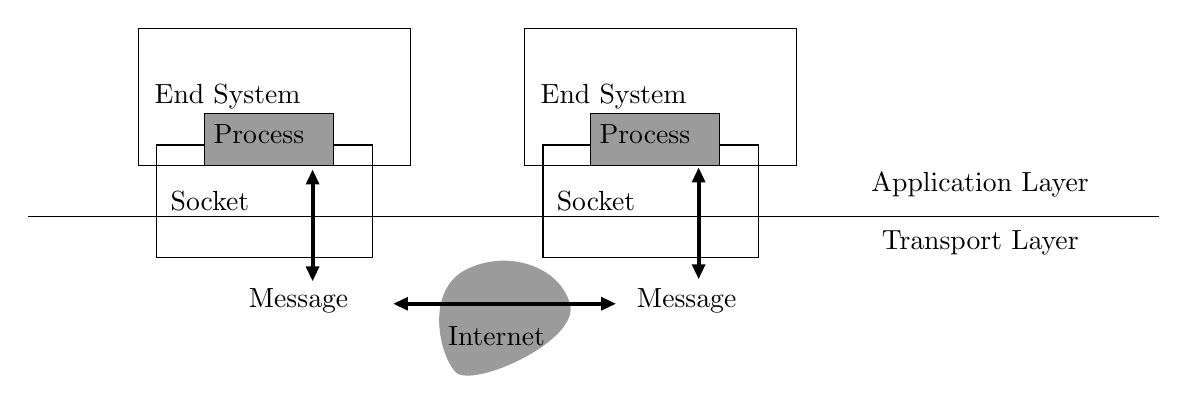
\begin{tikzpicture}[x=0.75pt,y=0.75pt,yscale=-1,xscale=1]
%uncomment if require: \path (0,300); %set diagram left start at 0, and has height of 300

%Shape: Polygon Curved [id:ds11925602136065394] 
\draw  [draw opacity=0][fill={rgb, 255:red, 155; green, 155; blue, 155 }  ,fill opacity=1 ] (233,228) .. controls (253,218) and (278,226.5) .. (283,244.5) .. controls (288,262.5) and (236,285.5) .. (228,277.5) .. controls (220,269.5) and (213,238) .. (233,228) -- cycle ;


%Straight Lines [id:da3659582184864416] 
\draw    (22,202.5) -- (567,202.5) ;
%Straight Lines [id:da934939440783863] 
\draw [line width=1.5]    (159,229.5) -- (159,184) ;
\draw [shift={(159,180)}, rotate = 90] [fill={rgb, 255:red, 0; green, 0; blue, 0 }  ][line width=0.08]  [draw opacity=0] (6.97,-3.35) -- (0,0) -- (6.97,3.35) -- cycle    ;
\draw [shift={(159,233.5)}, rotate = 270] [fill={rgb, 255:red, 0; green, 0; blue, 0 }  ][line width=0.08]  [draw opacity=0] (6.97,-3.35) -- (0,0) -- (6.97,3.35) -- cycle    ;
%Straight Lines [id:da2052672189764062] 
\draw [line width=1.5]    (345,228.5) -- (345,183) ;
\draw [shift={(345,179)}, rotate = 90] [fill={rgb, 255:red, 0; green, 0; blue, 0 }  ][line width=0.08]  [draw opacity=0] (6.97,-3.35) -- (0,0) -- (6.97,3.35) -- cycle    ;
\draw [shift={(345,232.5)}, rotate = 270] [fill={rgb, 255:red, 0; green, 0; blue, 0 }  ][line width=0.08]  [draw opacity=0] (6.97,-3.35) -- (0,0) -- (6.97,3.35) -- cycle    ;
%Straight Lines [id:da006036444966908028] 
\draw [line width=1.5]    (202,244.5) -- (301,244.5) ;
\draw [shift={(305,244.5)}, rotate = 180] [fill={rgb, 255:red, 0; green, 0; blue, 0 }  ][line width=0.08]  [draw opacity=0] (6.97,-3.35) -- (0,0) -- (6.97,3.35) -- cycle    ;
\draw [shift={(198,244.5)}, rotate = 0] [fill={rgb, 255:red, 0; green, 0; blue, 0 }  ][line width=0.08]  [draw opacity=0] (6.97,-3.35) -- (0,0) -- (6.97,3.35) -- cycle    ;

% Text Node
\draw    (261,111.75) -- (392,111.75) -- (392,177.75) -- (261,177.75) -- cycle  ;
\draw (326.5,144.75) node   [align=left] {\begin{minipage}[lt]{86.36pt}\setlength\topsep{0pt}
End System
\end{minipage}};
% Text Node
\draw    (270,168) -- (374,168) -- (374,222) -- (270,222) -- cycle  ;
\draw (322,195) node   [align=left] {\begin{minipage}[lt]{68pt}\setlength\topsep{0pt}
Socket
\end{minipage}};
% Text Node
\draw  [fill={rgb, 255:red, 155; green, 155; blue, 155 }  ,fill opacity=1 ]  (293,153) -- (355,153) -- (355,178) -- (293,178) -- cycle  ;
\draw (296,157) node [anchor=north west][inner sep=0.75pt]   [align=left] {Process};
% Text Node
\draw    (75,111.75) -- (206,111.75) -- (206,177.75) -- (75,177.75) -- cycle  ;
\draw (140.5,144.75) node   [align=left] {\begin{minipage}[lt]{86.36pt}\setlength\topsep{0pt}
End System
\end{minipage}};
% Text Node
\draw    (84,168) -- (188,168) -- (188,222) -- (84,222) -- cycle  ;
\draw (136,195) node   [align=left] {\begin{minipage}[lt]{68pt}\setlength\topsep{0pt}
Socket
\end{minipage}};
% Text Node
\draw  [fill={rgb, 255:red, 155; green, 155; blue, 155 }  ,fill opacity=1 ]  (107,153) -- (169,153) -- (169,178) -- (107,178) -- cycle  ;
\draw (110,157) node [anchor=north west][inner sep=0.75pt]   [align=left] {Process};
% Text Node
\draw (427,180) node [anchor=north west][inner sep=0.75pt]   [align=left] {Application Layer};
% Text Node
\draw (432,208) node [anchor=north west][inner sep=0.75pt]   [align=left] {Transport Layer};
% Text Node
\draw (127,236) node [anchor=north west][inner sep=0.75pt]   [align=left] {Message};
% Text Node
\draw (314,236) node [anchor=north west][inner sep=0.75pt]   [align=left] {Message};
% Text Node
\draw (223,254) node [anchor=north west][inner sep=0.75pt]   [align=left] {Internet};


\end{tikzpicture}
\caption{套接字是应用程序和网络之间的 API}
\end{figure}

\subsubsection{进程寻址}

在一台主机上运行的进程为了向另一台主机上运行的进程发送分组, 接收进程需要有一个地址.
为了标识这个接收进程, 我们首先需要标识主机的地址, 其次, 还需要在目的主机中指定接收进程
的标识符.

在因特网中, 主机由其 \textbf{IP 地址} (IP Address) 标识, IP 地址是一个 32 比特的量,
它能够唯一地标识一台主机. 目的地\textbf{端口号} (port number) 用于标记目的主机上的
接收进程 (接受套接字).

\subsection{运输层协议}

很多网络都提供了不止一种运输层协议, 当开发一个应用时, 必须选择一种可用的运输层协议.
而选择合适的运输层协议的思路是, 判断它提供的服务是否能满足你的需求. 我们大体上, 将
应用程序的服务要求分为四类: 可靠数据传输、吞吐量、定时和安全性.

\subsubsection{可靠数据传输}

一个协议如果能通过某些工作确保{\kaishu 由应用程序的一端发送的数据能够正确并完全的交付给该应用程序的
另一端}, 那么该协议就提供了\textbf{可靠数据传输} (reliable data transfer) 的服务.

与需要可靠数据传输的应用相对的网络应用是\textbf{容忍丢失的应用} (loss-tolerant application),
这些应用能够承受一定程度的数据损失.

\subsubsection{吞吐量}

某些应用程序对吞吐量是有要求的, 这些应用称为\textbf{带宽敏感应用} (bandwidth-sensitive application),
带宽敏感应用需要选择那些{\kaishu 能够以某种特定的速率提供确保的可用吞吐量}的运输层协议,
这就是说, 当应用程序请求 $r \si{bps}$ 的确保吞吐量时, 该运输层协议能够确保可用的
吞吐量总是大于等于 $r \si{bps}$.

与带宽敏感应用相对的是\textbf{带宽弹性应用} (bandwidth-elastic application),
这些应用能够根据当前可用带宽来可变地调整吞吐量.

\subsubsection{定时}

我想你在打在线游戏的时候最不想看到的就是屏幕左上角 (或者右上角) 的连接指示灯变成橙色或者
红色, 然后时延变成 $999 \si{ms}$. 这些网络应用需要选择能够提供定时保证的运输层协议,
当然了, 协议也不是万能的, 有的时候尽管选择了提供定时保证的协议, 但是你打游戏还是会卡.

你可能会在想, 我打游戏经常卡成这样, 凭什么你还敢说这是一个保证定时通信的协议?
这是不是虚假宣传? 我们说, 不是的. 这是因为, 虽然作为个人来看, 在打游戏的时候确实
时常会遇到卡顿的现象, 但是在整个互联网当中, 这个卡顿线性的发生频率就相当低了,
那么自然可以说这是一个 “保证定时” 的协议.

\subsubsection{安全性}

有的运输协议能够提供一种或多种安全性服务, 最简单的一个例子是, 是网络信息传输中的信息加密.
顺带一提, QQ 和微信的信息加密等级非常之低.

\subsection{TCP 和 UDP}

因特网为应用程序提供了两个运输层协议——TCP 和 UDP.

\subsubsection{TCP 服务}

TCP 服务模型包括面向连接服务和可靠数据传输服务.
\begin{itemize}[itemsep=0pt]
    \item \textbf{面向连接的服务}: 握手 (建立连接) —— 传输数据 —— 拆除连接.
    在数据报文开始流动之前, TCP 让客户和服务器相互交换运输层控制信息, 在握手阶段后,
    一个 \textbf{TCP 连接} (TCP connection) 就在两个进程的套接字之间建立了.
    连接双方的进程在此链接上同时进行报文收发, 在报文结束发送后, 连接被拆除.
    \item \textbf{可靠数据传输服务}: 通信进程能够依靠 TCP, 无差错、按适当顺序地交付
    所有发送的数据, 而没有字节的丢失或冗余.
\end{itemize}

此外, TCP 还具有拥塞控制机制. 当发送方和接收方之间的网络出现拥塞时,
TCP 的拥塞控制机制会抑制发送进程.

\subsubsection{UDP 服务}

UDP 是一种不提供不必要服务的轻量级运输协议, 它仅提供最低限度的服务. 它的主要特点为:
\begin{itemize}[itemsep=0pt]
    \item 无连接: 在两个进程通信前并没有握手过程.
    \item 不可靠数据传输: 当进程将一个报文发送斤 UDP 套接字时, UDP 并不保证该报文将到达
    接收进程, 不仅如此, 到达接收进程的报文也可能是乱序到达的.
    \item 不包括拥塞机制: 因此 UDP 的发送端可以用它选定的任何速率向网络层注入数据.
\end{itemize}

\vspace*{1em}
今天的因特网能够为时间敏感应用提供满意的服务, 但它不能提供任何定时或吞吐量保证.

\subsection{应用层协议}

\textbf{应用层协议} (application-layer protocol) 规定了运行在不同的端系统上的
应用程序进程如何相互传递报文. 应用层协议定义了以下内容:
\begin{enumerate}[label={${\arabic*}^\circ$}, itemsep=0pt]
    \item 交换的报文类型. 例如请求报文和相应报文.
    \item 交换报文类型的语法. 例如报文中的各个字段以及这些字段是如何描述的.
    \item 字段的语义. 即这些字段中信息的含义.
    \item 一个进程何时发送报文、如何发送报文、按照什么样的规则对报文进行相应.
\end{enumerate}

\section{Web 和 HTTP}

\chapter{运输层}

\section{面向连接的运输: TCP}

\subsection{TCP 连接}

\subsubsection{TCP 的特征}

\begin{enumerate}[label={${\arabic*}^\circ$}, itemsep=0pt]
    \item 面向连接: 一个应用进程开始与另一个应用进程通信和发送数据之前,
    必须要建立 TCP 连接, 因此 TCP 是 \textbf{面向连接} 的 (connection-oriented).
    TCP 连接是一种逻辑连接, 其共同状态仅保留在两个通信端系统的 TCP 程序中.
    \item 全双工: TCP 连接提供的是 \textbf{全双工服务} (full-duplex service), 即两台建立了 TCP 连接的主机
    可以同时向对方发送数据.
    \item \textbf{点对点} (point-to-point): 一个 TCP 连接只连接一对主机.
\end{enumerate}

\subsubsection{TCP 连接的建立: 三次握手}

假设某台主机上的一个进程 (我们将其称为客户进程) 想要与另一台主机上的一个进程
(我们将其称为服务器进程) 建立 TCP 连接. 这时, 客户首先发送一个特殊的 TCP 报文段,
服务器用另一个特殊的报文段来响应.
这两个报文段不承载 “有效载荷”, 即不包含应用层数据, 它们的交换意味着这两台主机已经为
大量的报文段的通信做好了准备. 最后, 客户用第三个可以承载有效载荷的特殊报文段作为第二个
报文段的响应, TCP 连接上的通信正式开始. 这一过程被称为\textbf{三次握手}
(three-way handshake).

\begin{figure}[H]
    \centering


\tikzset{every picture/.style={line width=0.75pt}} %set default line width to 0.75pt        

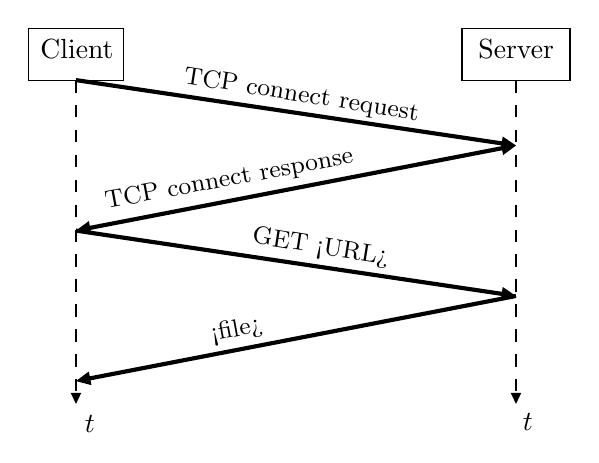
\begin{tikzpicture}[x=0.75pt,y=0.75pt,yscale=-1,xscale=1]
%uncomment if require: \path (0,300); %set diagram left start at 0, and has height of 300

%Straight Lines [id:da39916859175456754] 
\draw  [dash pattern={on 4.5pt off 4.5pt}]  (431,71) -- (431,224) ;
\draw [shift={(431,227)}, rotate = 270] [fill={rgb, 255:red, 0; green, 0; blue, 0 }  ][line width=0.08]  [draw opacity=0] (5.36,-2.57) -- (0,0) -- (5.36,2.57) -- cycle    ;
%Straight Lines [id:da9619721769875587] 
\draw  [dash pattern={on 4.5pt off 4.5pt}]  (219,71) -- (219,224) ;
\draw [shift={(219,227)}, rotate = 270] [fill={rgb, 255:red, 0; green, 0; blue, 0 }  ][line width=0.08]  [draw opacity=0] (5.36,-2.57) -- (0,0) -- (5.36,2.57) -- cycle    ;
%Straight Lines [id:da7790367004301654] 
\draw [line width=1.5]    (219,71) -- (427.04,101.91) ;
\draw [shift={(431,102.5)}, rotate = 188.45] [fill={rgb, 255:red, 0; green, 0; blue, 0 }  ][line width=0.08]  [draw opacity=0] (6.97,-3.35) -- (0,0) -- (6.97,3.35) -- cycle    ;
%Straight Lines [id:da886185187214201] 
\draw [line width=1.5]    (222.93,142.74) -- (427.07,103.26) ;
\draw [shift={(431,102.5)}, rotate = 169.05] [fill={rgb, 255:red, 0; green, 0; blue, 0 }  ][line width=0.08]  [draw opacity=0] (6.97,-3.35) -- (0,0) -- (6.97,3.35) -- cycle    ;
\draw [shift={(219,143.5)}, rotate = 349.05] [fill={rgb, 255:red, 0; green, 0; blue, 0 }  ][line width=0.08]  [draw opacity=0] (6.97,-3.35) -- (0,0) -- (6.97,3.35) -- cycle    ;
%Straight Lines [id:da3209107668447636] 
\draw [line width=1.5]    (219,143.5) -- (427.04,174.41) ;
\draw [shift={(431,175)}, rotate = 188.45] [fill={rgb, 255:red, 0; green, 0; blue, 0 }  ][line width=0.08]  [draw opacity=0] (6.97,-3.35) -- (0,0) -- (6.97,3.35) -- cycle    ;
%Straight Lines [id:da9506908059835723] 
\draw [line width=1.5]    (222.93,215.24) -- (431,175) ;
\draw [shift={(219,216)}, rotate = 349.05] [fill={rgb, 255:red, 0; green, 0; blue, 0 }  ][line width=0.08]  [draw opacity=0] (6.97,-3.35) -- (0,0) -- (6.97,3.35) -- cycle    ;

% Text Node
\draw    (196,46) -- (242,46) -- (242,71) -- (196,71) -- cycle  ;
\draw (199,50) node [anchor=north west][inner sep=0.75pt]   [align=left] {\begin{minipage}[lt]{28.8pt}\setlength\topsep{0pt}
\begin{center}
Client
\end{center}

\end{minipage}};
% Text Node
\draw    (405,46) -- (457,46) -- (457,71) -- (405,71) -- cycle  ;
\draw (408,50) node [anchor=north west][inner sep=0.75pt]   [align=left] {\begin{minipage}[lt]{32.77pt}\setlength\topsep{0pt}
\begin{center}
Server
\end{center}

\end{minipage}};
% Text Node
\draw (433,230.4) node [anchor=north west][inner sep=0.75pt]    {$t$};
% Text Node
\draw (222,231.4) node [anchor=north west][inner sep=0.75pt]    {$t$};
% Text Node
\draw (270.91,62.91) node [anchor=north west][inner sep=0.75pt]  [font=\small,rotate=-9.08] [align=left] {TCP connect request};
% Text Node
\draw (230.81,123.89) node [anchor=north west][inner sep=0.75pt]  [font=\small,rotate=-349.48] [align=left] {TCP connect response};
% Text Node
\draw (303.91,139.91) node [anchor=north west][inner sep=0.75pt]  [font=\small,rotate=-9.08] [align=left] {GET <URL>};
% Text Node
\draw (281.81,187.54) node [anchor=north west][inner sep=0.75pt]  [font=\small,rotate=-349.48] [align=left] {<file>};


\end{tikzpicture}
\caption{三次握手}
\end{figure}

\subsubsection{TCP 如何传送数据}

\begin{enumerate}[label={${\arabic*}^\circ$}, itemsep=0pt]
    \item 客户进程将数据通过套接字送入运输层, 交由 TCP 控制.
    \item TCP 将这些数据引导到该连接的 \textbf{发送缓存} (send buffer) 中.
    \item TCP 不时从发送缓存中取出一块数据, 配上一个 \textbf{TCP 首部}
    (TCP header) 封装成 \textbf{TCP 报文段} (TCP segment) 传递到网络层,
    TCP 只负责报文段的逻辑传递, 而底层的物理传递则由下层的网络层、数据链路层和物理层来实现.
    \item 另一台主机上的 TCP 接收到一个报文段后, 将其放入 \textbf{接收缓存} 
    (receive buffer) 中.
    \item 应用程序从接收缓存中读取数据流.
\end{enumerate}

\newpage
\thispagestyle{empty}

\chapter{网络层: 数据平面}



\section{网络层概述}

网络层能够被分解为两个相互作用的部分, 数据平面和控制平面.

\subsection{转发和路由选择: 数据平面和控制平面}

网络层的数据平面的功能, 即\textbf{转发}功能, 是网络层中每台路由器的功能, 该数据平面功能决定到达路由器输入链路
之一的数据报 (即网络层分组) 如何转移到该路由器的输出链路之一.

具体转移到哪一个输出链路,
则根据\textbf{转发表}的值来确定, 转发表是一台路由器的路由选择算法与其他路由器的路由选择算法进行通信
和计算得到的.

控制平面功能, 即\textbf{路由}功能, 控制数据报沿着从源主机到目的主机的端到端路径中路由器之间
的路由方式, 决定了端到端传输的数据路径.

每台路由器的数据平面的主要作用是从其输入链路向其输出链路转发数据报, 控制平面的主要作用是
协调这些本地的路由器的转发操作, 使得数据报沿着源和目的主机之间的路由器路径最终进行端到端
传送.

\subsection{网络层分组 \quad 分组交换机 \quad 路由器}

“分组” 这一概念在 TCP/IP 体系结构模型的不同层次中用不同的术语来表达.
运输层分组的名字是报文段 (segment\footnote{
    读作 /segmənt/.
}), 数据链路层的分组称为帧 (frame), 而网络层的分组称为
网络层\textbf{数据报} (datagram). 数据报对报文段进行了一次拆分, 使其具有
更小的体积, 同时附上了网络层首部 $\mathrm{H_n}$, 而链路层帧则是对网络层数据报
的又一次拆封和封装, 附上了链路层首部 $\mathrm{H_l}$.

分组交换机一词在计算机网络中可以指代路由器, 也可以指链路层交换机.
在进行转发时, 链路层交换机通过链路层帧中的字段值来进行决策, 而路由器
则基于网络层数据报中的首部字段值决策.

\subsection{因特网的服务模型}

因特网的网络层服务模型是一种\textbf{尽力而为} (best-effort) 的服务, 这就是说,
它并不保证数据的可靠传输、并不保证数据报的顺序到达, 在带宽、延迟等方便也不做任何的保证.

\appendix
% 设置 chapter 标题样式
\titleformat{\chapter}[hang]{\centering\heiti\Large\bfseries}{附录\,\thechapter}{1em}{}
\renewcommand{\chaptermark}[1]{\markboth{附录 \thechapter\, #1}{}}

\begin{thebibliography}{1}
    \addcontentsline{toc}{chapter}{参考文献}
    \bibitem{自顶向下}
    [美] James F.Kurose, [美] Keith W. Ross. 计算机网络: 自顶向下方法
    (Computer Networking: A Top Down Approach, 8e)[M]. 
    陈鸣译. 北京: 机械工业出版社, 2022.
    \bibitem{王道计网}
    王道论坛组. 2024 年计算机网络考研复习指导 [M]. 北京: 电子工业出版社, 2022.
\end{thebibliography}

\newpage
\thispagestyle{empty}
\vspace*{5cm}
\begin{center}
    \includegraphics*[width=\textwidth]{pic/i_love_npu.jpeg}
    \large
    公诚勇毅 \quad 永矢毋忘

    中华灿烂 \quad 工大无疆
\end{center}
\vspace*{13em}
\begin{center}
    \small
    本文档由\textbf{钱锋}编写, 钱锋保留一切权利.

    文档中出现的部分素材来源于网络, 笔者承诺这些素材仅供学习交流之用, 
    它们的原作者保留一切权利.

    2023 年 \quad 西北工业大学 \quad 中国西安 
\end{center}

\end{document}